\documentclass[a4paper,11pt]{article}
\pdfoutput=1 % if your are submitting a pdflatex (i.e. if you have images in pdf, png or jpg format)

\usepackage{jcappub} % for details on the use of the package, please
                 % see the JCAP-author-manual

\usepackage{hyperref}
\usepackage{amsmath}

%\usepackage[english,activeacute]{babel} 
\usepackage[toc,page]{appendix}
\usepackage{graphicx}
\usepackage{color}
\usepackage{tensor}

\usepackage{xcolor}
\usepackage{graphicx}
\usepackage{colortbl}
\usepackage{placeins}
\usepackage[margin=2.5cm]{geometry}
\usepackage{multirow}

\usepackage[utf8]{inputenc}

% command for co-polarized
\newcommand{\co}{\mathbin{\|}}

% command for cross-polarized
\newcommand{\cx}{\mathbin{\times}}


\title{\boldmath Pixel space convolution for cosmic microwave background experiments}


%% %simple case: 2 authors, same institution
%% \author{A. Uthor}
%% \author{and A. Nother Author}
%% \affiliation{Institution,\\Address, Country}

% more complex case: 4 authors, 3 institutions, 2 footnotes
\author[a]{P. Flux\'a, }
\author[b]{M.K. Brewer, }
\author[a]{R. D\"unner.}

% The "\note" macro will give a warning: "Ignoring empty anchor..."
% you can safely ignore it.

\affiliation[a]{Instituto de Astrof\'isica, Pontificia Universidad Cat\'olica de Chile ,\\Vicu\~na Mackenna 4860, Chile}
\affiliation[b]{Department of Astronomy, Johns Hopkins University,\\Baltimore MD, USA}

% e-mail addresses: one for each author, in the same order as the authors
\emailAdd{pedro@fluxanet.net}
\emailAdd{brewer@astro.umass.edu}
\emailAdd{rdunner@astro.puc.cl}


\abstract{
Cosmic microwave background experiments have experienced an exponential increase in complexity, data size and sensitivity. One of the goals of current and future experiments is to characterize the B-mode power spectrum, which would be considered a strong evidence supporting inflation. The signal associated with inflationary B-modes is very weak, and so a successful detection requires exquisite control over systematic effects, several of which might arise due to the interaction between the electromagnetic properties of the telescope beam, the scanning strategy and the sky model. In this work, we present the Pixel Space COnvolver (PISCO), a new software tool capable of producing mock data streams for a general CMB experiment. PISCO uses a fully polarized representation of the electromagnetic properties of the telescope. PISCO also exploits the massively parallel architecture of Graphic Processing Units to speed-up the main calculation. This work shows the results of applying PISCO in several scenarios, included a realistic simulation of an ongoing experiment, the Cosmology Large Angular Scale Surveyor.}


%\abstract{
%	Cosmic microwave background experiments have experienced an exponential increase in complexity, data size and sensitivity. Current and future experiments aim at characterizing the B-mode power spectrum which, due to its faintness, will require extreme control over systematic effects. One such effect might arise from the complex coupling between the telescope beam and its scanning strategy. In this work, we present a new software tool, the Pixel Space COnvolver, PISCO, capable of producing mock data streams for a general CMB experiment. We show results of an application of PISCO to the Cosmology Large Angular Scale Surveryor, and its Q-band telescope.  }

\begin{document}
\maketitle
\flushbottom

% enable numbering of equations that considers the section number
%\numberwithin{equation}{section}

\section{Introduction}

% gives the width of the current document in pts
%	\showthe\textwidth

The study of the cosmic microwave background (CMB) in the last few decades has lead to major advances in Cosmology. In particular, the study of the temperature and polarization anisotropy field has allowed us to achieve percent level constraints on cosmological parameters, favoring a universe dominated by cold dark matter plus a cosmological constant ($\Lambda$CDM), known today as the standard model of Cosmology (see \cite{2016A&A...594A..12P}). Current efforts are mostly focused on the polarization anisotropy field, as it promises to provide independent constraints on the very early stages of the Universe. At these very first moments, the leading theory predicts that the Universe exponentially expanded nearly 60 e-folds in a process called inflation, becoming the flat, homogeneous and isotropic Universe that we see today. If true, gravitational waves generated by this expansion would have later interacted with the surface of last scatter, leaving a unique imprint in the polarization field which should be observable today.

Electromagnetic radiation from the CMB anisotropy field is nearly 10\% polarized. These polarized anisotropies can be modeled as a spin-2 field, which is separable in two orthogonal components: a curl-free component called E-mode, and a divergence-free component called B-mode. In the absence of gravitational waves, the polarization field would contain only E-modes, which would be partially turned into B-modes by gravitational lensing. The resulting B-mode field would be one or more orders of magnitude lower than the E-mode signal, being very faint and difficult to measure. Moreover, recent results show that this signal lies below other polarized emissions, like the interstellar medium (see \cite{2018PhRvL.121v1301B}), indicating that detection of the primordial B-mode signal is indeed a major technical challenge.

Another source of confusion is experimental systematic effects. The tremendous increase in sensitivity of CMB experiments has brought into play a long list of instrumental and observational effects, which need to be properly incorporated not only into the data reduction process, but into the design of future experiments as well. Because the CMB is an extended signal on the sky, it is crucial to characterize the beam, or in the more general case, the polarized antenna response of the telescope. It is also key to model and understand how this response gets convolved with the sky signal via the given scanning strategy, as this process may directly affect the scientific results.

%The main beam is where most of the radiation is captured by the antenna, and thus the effects of the beam shape and polarization have been extensively studied. 
%Analytic techniques
Modeling the effect of the telescope beam on scientific results can be done analytically or numerically. For instance, the effect of symmetrical beams with smooth profiles can be analytically accounted for when computing the power spectra of CMB maps (see \cite{2003ApJS..148...39P}). The impact of other related systematic effects, like beam mismatch, has also been described in the literature (see \cite{PhysRevD.77.083003, 2007MNRAS.376.1767O, 2015JCAP...03..048D}). When the beam has more complex features, like sidelobes, numerical methods must be used instead. Several techniques that rely on harmonic space representations of the beam, the sky and the scanning strategy have been devised (see \cite{2001PhRvD..63l3002W,2000PhRvD..62l3002C}). An excellent description of an implementation of this is given in \cite{2018arXiv180905034D}. Another approach is the one followed by FeBeCop (see \cite{2011ApJS..193....5M}), which computes an effective beam instead of convolving the sky for every time sample. 

%Planks approach ... 
%The Planck experiment developed Full Focal Plane (FFP) simulations (see \cite{2016A&A...594A..12P}). At the time they were performed, FFP simulations took more than four million CPU-hours on a world-class supercomputer, and required almost 18 TB of storage. FFP simulations included very detailed noise models of the Planck mission and helped, among other things, to provide excellent constraints on the the cosmological parameters and their associated statistical errors (see \cite{2016A&A...594A..13P}). FFP simulations showed that effort on improving tools aimed at simulating CMB experiments will become valuable for current and future missions.

%O'dea approach ...

In this work, we describe the algorithm and prototype implementation of a new CMB computer simulation code, the Pixel Space COnvolver (PISCO). PISCO has the capability of accounting for arbitrary shaped, time-varying beams and sky models. Polarization properties of the beam are handled following the work presented in \cite{2007MNRAS.376.1767O}. PISCO also exploits the massively parallel architecture that Graphics Processing Units (GPU) provide via the CUDA application programming interface, and was designed from scratch to take advantage of HPC environments.

This paper is organized as follows. 
\S\ref{sec::coordinate-systems} contains a description of the coordinate system and geometrical transformations used to model an antenna pointing at the sky.
\S\ref{sec::antennas} and \S\ref{sec::convolution} describe the methodology that was used to model the polarizing properties of an antenna and its coupling to the sky.
\S\ref{sec::pisco} describes the algorithm used by PISCO, as well as a prototype implementation. 
\S\ref{sec::validation} presents validation tests on the prototype implementation of PISCO. 
\S\ref{sec::realistic_cmb_experiment} provides an example application of PISCO to the Cosmology Large Angular Scale Surveyor, CLASS (\cite{2016SPIE.9914E..1KH}). 
The paper concludes with a brief discussion of the results obtained in \S\ref{sec::conclusions}.

%
\section{Coordinates}
\label{sec::coordinate-systems}

\begin{figure*}
	\centering
	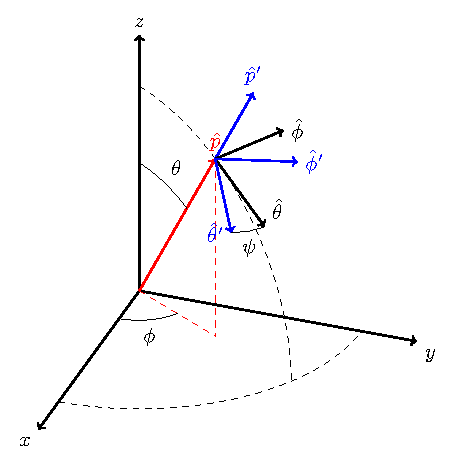
\includegraphics[width=0.47\linewidth]{tikz/sky_basis}	
	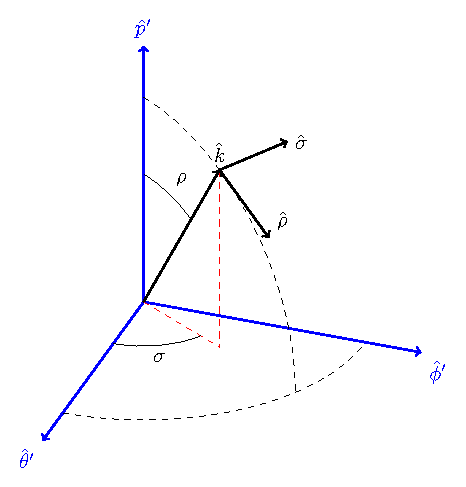
\includegraphics[width=0.47\linewidth]{tikz/beam_basis}
	\caption{Left panel: sky basis. The sky basis is a generic spherical coordinate system. $\hat{x}$, $\hat{y}$ and $\hat{z}$ form an orthonormal basis. Unit vector $\hat{p}$ is defined by its spherical coordinates, co-latitude $\theta$ and longitude $\phi$. Co-latitude increases from the north pole towards the south pole. Longitude increases from west to east. Tangent vectors at $\hat{p}$, $\hat{\theta}$ and $\hat{\phi}$, can be rotated around $\hat{p}$ by angle $\psi$ to generate vectors $\hat{\theta}'$ and $\hat{\phi}'$. Note an observer looking towards the sky along $\hat{p}$ will measure angle $\psi$ as increasing clockwise from South. Right panel: the antenna basis is built using spherical unit vectors $\hat{\theta}'$, $\hat{\phi}'$ and $\hat{p}'$, analogous to Cartesian unit vectors $\hat{x}$, $\hat{y}$ and $\hat{z}$. The orientation of the antenna basis with respect to the sky basis is completely determined by the pointing vector $\hat{p}$ and rotation angle $\psi$. A unit vector $\hat{k}$ in the antenna basis is described by $\rho$ (co-latitude) and $\sigma$ (longitude). Tangent vectors at $\hat{k}$ are $\hat{\rho}$ and $\hat{\sigma}$. }
	\label{fig::sky_basis} 
\end{figure*}

Since PISCO performs the convolution of the polarized antenna response with the sky in the spatial domain, it makes extensive use of coordinate transformations. These operations can be described by the use of two complementary spherical coordinate systems, which are described in Figure \ref{fig::sky_basis}. The first coordinate system corresponds to the \textsl{sky basis}. Unit base vectors of these coordinate system are $\hat{x}$, $\hat{y}$ and $\hat{z}$. For convenience, the antenna pointing in the sky basis will be described as a 3-tuple $\bar{q}$, so that an antenna aiming at co-latitude $\theta_0$ and longitude $\phi_0$, with position angle $\psi_0$ has a pointing 

\begin{equation}
\begin{aligned}
\bar{q}_0= (\theta_0,\phi_0,\psi_0) \, \rm{.}
\end{aligned}
\end{equation}

Then the \textsl{pointing direction}, denoted by vector $\hat{p}_0$, can be expressed as a linear combination of base vectors and spherical coordinates $(\theta_0,\phi_0)$ via

\begin{equation}
\begin{aligned}
\hat{p}_0 = \sin(\theta_0)\cos(\phi_0) \hat{x} + \sin(\theta_0)\sin(\phi_0) \hat{y} + \cos(\theta_0) \hat{z} \, \rm{.}
\end{aligned}
\label{eq::p_sky_basis}
\end{equation}

The vectors $\hat{\theta}_0$ and $\hat{\phi}_0$ are computed using

\begin{eqnarray}
\begin{aligned}
\hat{\theta}_0 &=&  \cos(\theta_0) \cos(\phi_0) \hat{x} + \cos(\theta_0)\sin(\phi_0) \hat{y} - \sin(\theta_0) \hat{z} \\
\hat{\phi}_0   &=&              -\sin(\phi_0) \hat{x} +             \cos(\phi_0) \hat{y} \, \rm{.}
\end{aligned}
\label{eq::tangent_sky_basis}
\end{eqnarray}

These vectors can be used to build a second coordinate system, the \textsl{antenna basis}. Given an antenna pointing $\bar{q}_0$, the antenna basis base vectors can be written in term of sky basis coordinates as 

\begin{eqnarray}
%\begin{aligned}
\hat{p}'_0      &=&  \hat{p}_0 \\
\hat{\theta}'_0 &=&  \cos(\psi_0)\hat{\theta}_0 + \sin(\psi_0)\hat{\phi}_0 \\
\hat{\phi}'_0   &=& -\sin(\psi_0)\hat{\theta}_0 + \cos(\psi_0)\hat{\phi}_0 \, \rm{.}
%\end{aligned} 
\label{eq::antenna_base_vectors}
\end{eqnarray}

In the antenna basis, coordinates analog to sky basis co-latitude and longitude are $\rho$ and $\sigma$, respectively. As in equation \ref{eq::p_sky_basis}, a vector $\hat{k}$ can be similarly written in terms of antenna basis coordinates as

\begin{equation}
\begin{aligned}
\hat{k}       &=&  \sin(\rho)\cos(\sigma)\hat{\theta}'_0 + \sin(\rho)\sin(\sigma) \hat{\phi}'_0 + \cos(\rho) \hat{p}'_0 
\end{aligned}
\end{equation}

\noindent
while vectors analog to the ones described by equation \ref{eq::tangent_sky_basis} are

\begin{eqnarray}
\begin{aligned}
\hat{\rho}    &=&  \cos(\rho)\cos(\sigma)\hat{\theta}'_0 + \sin(\rho)\sin(\sigma) \hat{\phi}'_0 - \sin(\rho) \hat{p}'_0 \\
\hat{\sigma}  &=& -\sin(\sigma)\hat{\theta}'_0 + \cos(\sigma)\hat{\phi}'_0 \, \rm{.}
\end{aligned}
\end{eqnarray}

In many situations, antennas are equipped with polarization sensitive devices. The direction on the sky for which the device has maximum sensitivity to linearly polarized radiation is called co-polarization, denoted by $\hat{e}_{\co}$. The perpendicular direction, known as cross-polarization, is denoted by $\hat{e}_{\cx}$.
Because polarization is defined in the sky basis (see Figure \ref{fig::cmbcoordconvention}), a polarization sensitive antenna must compensate for the apparent rotation of its own polarization basis with respect to the sky. This can be accomplished by rotating the incoming Stokes vector by the angle between $\hat{e}_{\co}$ and $\hat{\theta}$, namely

\begin{equation}
\chi(\rho,\sigma) = \arctan \left( \frac{ |\hat{e}_{\co} \times \hat{\theta}| }{ \hat{e}_{\co} \cdot \hat{\theta} } \right) \, \rm{.}
\label{eq::psi}
\end{equation}

See Appendix A for details on the definition of co-polarization and cross-polarization that PISCO uses and the computation of $\chi(\rho,\sigma)$ using spherical trigonometry.

\begin{figure}
	\centering
	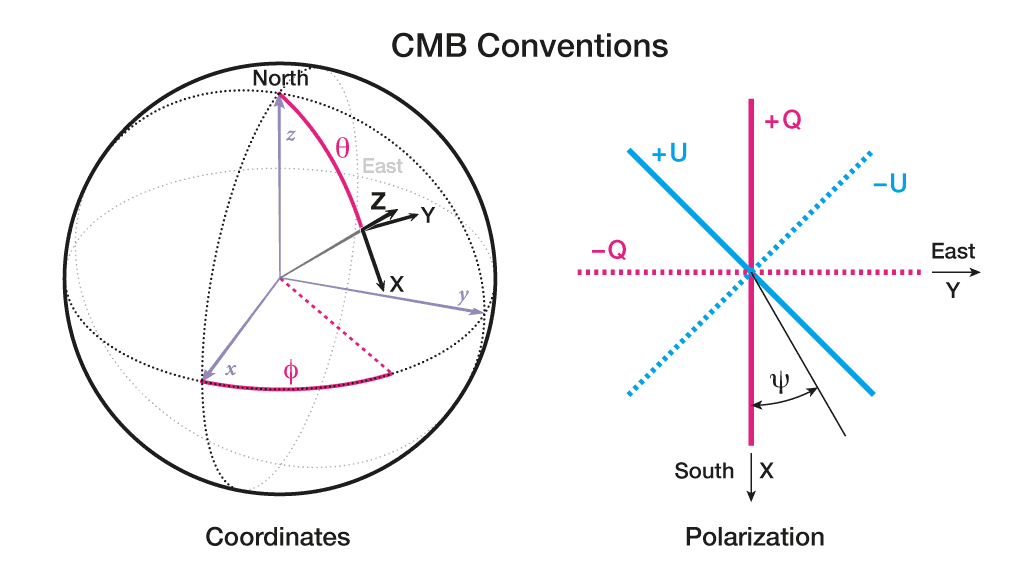
\includegraphics[width=0.7\linewidth]{figures/cmb_coord_convention}
	\caption{Figure showing the convention used for polarization among the CMB community. In this figure, $z$ is parallel to $\hat{p}_0$, $x$ is parallel to $\hat{\theta}$ and $y$ points along $\hat{\phi}$. $\psi$ is the angle between the antenna ``up'' direction, and $x$ ($\hat{\theta}$). The sign conventions of Stokes parameters $Q$ and $U$ used by the CMB community are: positive $Q$ if the polarization vector is aligned with $\hat(\theta)$ (North-South direction), negative $Q$ if the polarization vector is aligned with $\hat{\phi}$ (East-West direction), positive $U$ is aligned with $(\pm(\hat{\phi} + \hat{\theta})/\sqrt{2} )$ (North/West-South/East direction), and negative $U$ is aligned with $(\pm(\hat{\phi} - \hat{\theta})/\sqrt{2} )$ (North/East-South/West direction). Note that the right-most panel of this figure corresponds to an observer looking \textsl{towards Earth}. Figure source: \href{https://lambda.gsfc.nasa.gov/product/about/pol_convention.cfm}{LAMBDA website}}
	\label{fig::cmbcoordconvention}
\end{figure}

\section{A polarized model for antennas}
\label{sec::antennas}

The properties of an antenna equipped with detectors that are insensitive to polarization can be fully characterized by its beam. The beam is defined in terms of the antenna angular power density distribution $U(\rho,\sigma)$ via

\begin{equation}
\begin{aligned}
\mathit{b}(\rho, \sigma) = \frac{ U(\rho, \sigma) }{ \mathrm{max}\left[ U(\rho,\sigma) \right] }  =  \frac{ U(\rho, \sigma) }{ U(0,0) } \, .
\end{aligned}
\label{eq::beam_def}
\end{equation}

\noindent
From this definition of the beam, a standard quantification of an antenna's ability to direct power to a particular region of the sky is given by the beam solid angle $\Omega$, calculated as

\begin{equation}
\begin{aligned}
\Omega = \int_{4\pi} \mathit{b}(\rho,\sigma) \, \mathrm{d} \Omega \, .
\end{aligned}
\label{eq::omega_def}
\end{equation}

\noindent
These concepts fully characterize a lossless antenna in the case it is not sensitive to polarization, while modern CMB experiments, aim at measuring E-modes and B-modes. It then becomes necessary to introduce a more general treatment of the antenna, so as to include its polarizing properties. 

%This orientation can be parameterized in terms of an angle $\zeta$, which is the angle between the orientation of the polarization sensitivity axis of one detector and $\hat{\theta}^{\prime}_0$.

Many CMB experiments use polarization sensitive bolometers (PSBs) as detection devices, which are pairs of bolometers placed at the focus of the optical chain. By construction, each bolometer is more sensitive to a particular orientation of incoming electric fields. Given a PSB consisting of a pair of detectors $(a,b)$ whose polarization sensitive axes are aligned at angles $\zeta$ and $\zeta - 90^{\circ}$ with respect to the antenna basis unit vector $\hat{\theta}'_0$, we can define beam center polarization unit vectors for each detector as

\begin{align}
\hat{e}_{a,{\co}}    &= \quad \cos(\zeta)\hat{\theta}'_0 + \sin(\zeta)\hat{\phi}'_0 \\
\hat{e}_{a,{\cx}}    &= \quad \sin(\zeta)\hat{\theta}'_0 - \cos(\zeta)\hat{\phi}'_0 \\
\hat{e}_{b,{\co}}    &= \quad \sin(\zeta)\hat{\theta}'_0 - \cos(\zeta)\hat{\phi}'_0 \\
\hat{e}_{b,{\cx}}    &= -\cos(\zeta)\hat{\theta}'_0 - \sin(\zeta)\hat{\phi}'_0 \, \rm{.} 
\label{eq::copol_bolo}
\end{align}


% PF: I had to comment this out because my LaTeX complains about "double subscript"
%\begin{align}
%\hat{e}_a_{\co}    &= \quad \cos(\zeta)\hat{\theta}'_0 + \sin(\zeta)\hat{\phi}'_0 \\
%\hat{e}_a_{\cx}    &= \quad \sin(\zeta)\hat{\theta}'_0 - \cos(\zeta)\hat{\phi}'_0 \\
%\hat{e}_b_{\co}    &= \quad \sin(\zeta)\hat{\theta}'_0 - \cos(\zeta)\hat{\phi}'_0 \\
%\hat{e}_b_{\cx}    &= -\cos(\zeta)\hat{\theta}'_0 - \sin(\zeta)\hat{\phi}'_0 \rm{.} \\
%\label{eq::copol_bolo}
%\end{align}

%\noindent
%Where the subscript $\co$ denotes ``co-polarization'' and $\cx$ to ``cross-polarization''. 

% removing conversely
%Conversely, polarizing
The polarizing properties of an antenna can be obtained by combining the concept of a beam with the Mueller matrix formalism. Mueller matrices are widely used to quantify the effect that an optical element has on the polarization state of incoming light. This process is modeled by the multiplication of $4\times4$ matrix $\mathbf{M}$ with a Stokes vector $S_{\mathrm{in}}$, such that the Stokes vector of radation that has interacted with the optical element becomes

\begin{equation}
\begin{aligned}
S_{\mathrm{out}} = \mathbf{M} S_{\mathrm{in}} \, .
\end{aligned}
\end{equation}

\noindent
As described in the work of \cite{piepmeier_long_njoku_2008} and \cite{2007MNRAS.376.1767O}, antennas can be modeled using Mueller matrices. PISCO uses the formalism presented in \cite{2007MNRAS.376.1767O}, since it is more suitable to be applied to CMB experiments. We note the original paper names ``beam Mueller fields'' to this extended definition of a antenna beam. To emphasize the multi-dimensional nature of this mathematical entity, in this work we refer to it as a beam tensor, or \textsl{beamsor} for short.

A beamsor can be interpreted as a field of Mueller matrices such that for each direction $(\rho,\sigma)$, there is an associated Mueller matrix that quantifies the coupling between the antenna and a Stokes vector coming from $(\rho,\sigma)$. We will denote a beamsor by letter $B = B(\rho,\sigma)$. At every antenna basis direction, $B$ is a $4\times4$ matrix in the form

\begin{equation}
\begin{aligned}
B(\rho,\sigma) = \frac{1}{\tilde{\Omega}}
\begin{bmatrix}
B_{TT} & B_{QT} & B_{UT} & B_{VT}\\
B_{TQ} & B_{QQ} & B_{UQ} & B_{VQ}\\
B_{TU} & B_{QU} & B_{UU} & B_{VU}\\
B_{TV} & B_{QV} & B_{UV} & B_{VV}
\end{bmatrix}
\end{aligned}
\label{eq::beamsor}
\end{equation}

\noindent
where $\tilde{\Omega}$ is a normalization factor given by

\begin{equation}
\begin{aligned}
\tilde{\Omega} = \int_{4\pi} B_{TT}(\rho,\sigma) \, \mathrm{d} \Omega
\end{aligned}
\end{equation}

\noindent
and the elements of $B$ are defined in the work of \cite{2007MNRAS.376.1767O}. Note that in the case of no cross polarization and perfectly matched beams, the beamsors reduces to the tensor product 

\begin{equation}
B(\rho,\sigma) = \mathit{b}(\rho,\sigma) \otimes \tensor{I}{}
\end{equation}

\noindent
where $\mathbf{I}$ an identity matrix. 

\section{Measuring the sky with polarization sensitive antennas}
\label{sec::convolution}
	
\subsection{Continuous case}

In order to model the process by which a polarization sensitive detector transforms electromagnetic radiation into current or voltage, we used the formalism described in \cite{2007A&A...470..771J}. In Mueller matrix space, a partially polarized, total power detection device corresponds to the following row-vector 

\begin{equation}
\begin{aligned}
\tensor{D}{_{i}}(\zeta,\epsilon,s) = \frac{s}{2} \left[(1 + \epsilon), (1 - \epsilon)\cos(2\zeta), (1 - \epsilon)\sin(2\zeta), 0 \right]
\end{aligned}
\label{eq::M_pol}
\end{equation}

\noindent
where $1 - \epsilon$ is the polarization efficiency, $s$ is the voltage responsivity of the detector and $\zeta$ was defined in Section \ref{sec::antennas}. The process of taking a total power measurement on a Stokes vector $\tensor{S}{^{i}}$ can then be modeled as a dot product which, using Einstein's summation convention, yields

\begin{equation}
\begin{aligned}
d = \tensor{D}{_{i}} \tensor{S}{^{i}} \, .
\end{aligned}
\label{eq::total_power_measurement}
\end{equation}

Stokes vector $\tensor{S}{^{i}}$ is, in turn, the convolution between the antenna beamsor and the polarized sky. The complete expression describing the measurement taken by a linearly polarized, total power detector coupled to an antenna pointing along $\hat{p}$ with position angle $\psi_0$ becomes

\begin{equation}
\begin{aligned}
d(\bar{q}_0) =  \int_{4\pi} \tensor{D}{_{i}}(\chi,\epsilon,s) \tensor{\Lambda}{^{i}_{l}}(\chi)  \tensor{B}{^{l}_{j} } \left[ \tensor{\Lambda}{^{j}_{m}}(-\chi) \tensor{S}{^{m}} \right ] \, \mathbf{d} \Omega 
\end{aligned}
\label{eq::pisco_equation_cont}
\end{equation}

\noindent
where $(i,j) = T,Q,U,V$, and $B$ is aligned with $(\hat{p},\psi_0)$. Rotation of the detector polarization basis to the sky basis is carried out using $\chi$ in the argument to $D$, and by $\Lambda$, which is a matrix field in the form

\begin{equation}
\begin{aligned}
\Lambda(\chi) =
\begin{bmatrix}
1  & 0 & 0 & 0\\
0  & \cos(2\chi) & -\sin(2\chi) & 0\\
0  &\sin(2\chi) & \cos(2\chi) & 0\\
0  & 0 & 0 & 1
\end{bmatrix}  \, \rm{.}
\end{aligned}
\label{eq::lambda_operator}
\end{equation}

\subsection{Pixelated case}
\label{sec::pixel_conv}

% removing this sentence:  It is worth noting that the TOD generation routine run by PISCO requires both the beamsor and sky model to be already pixelated. 
% as I believe it belongs to another subsection
In order to calculate the result of equation \ref{eq::pisco_equation_cont} using a computer, we can no longer use continuous distributions, so we need to use pixelated versions of both the beamsor and sky model. Both the sky model $S$ and beamsor $B$ must then be transformed into a matrix of $N_b$ (number of pixels in the beamsor) and $N_s$ (number of pixels in the sky model) entries, respectively. We will denote the $k$-th pixel of the pixelated beamsor $B$ (sky $S$) as $\tensor[_k]{B}{}$ ($\tensor[_k]{S}{}$). With the above in mind, we can write equation \ref{eq::pisco_equation_cont} for the pixelated case as

\begin{equation}
\begin{aligned}
d(\bar{q}_0) = \
\sum_{k=1}^{N_s} \
\tensor[_k]{D}{_{i}}(\chi,\epsilon,s) \
\tensor[_k]{\Lambda}{^{i}_{l}}(\chi) \
\tensor[_k]{B}{^l_j} \
\tensor[_k]{\Lambda}{^{j}_{m}}(-\chi) \
\tensor[_k]{S}{^m}  \, \rm{.}
\end{aligned}
\label{eq::discrete_beam_conv_tensor}
\end{equation}

\noindent
where $B$ has been properly re-pixelated via interpolation to be aligned with the sky according to $\bar{q}_0$ using the equations presented in Appendix A. It is worth noting that this expression operates on a pixelated sky, so information at angular scales that are smaller than a sky pixel is lost.

\section{PISCO}
\label{sec::pisco}

The \textbf{PI}xel \textbf{S}pace \textbf{CO}nvolver (PISCO) is a tool with the capability of generating synthetic Time Ordered Data (TOD) provided a model for the beamsor, the scanning strategy of the mission and a sky model. In this section, we present a pathfinder implementation of PISCO that exploits the massively parallel architecture of modern GPU systems.

\subsection{General description}

PISCO is the software tool in charge of generating mock TOD given a beamsor, a sky model and a scanning strategy. A diagram showing the general workings of PISCO is shown in Figure \ref{fig::pisco_flow}. PISCO receives as input a sky model in the form of 4 maps representing Stokes parameters $I,Q,U$ and $V$, a beamsor, pointing and focal plane information. PISCO stores the beamsor elements and sky model as HEALPix (see \cite{2005ApJ...622..759G}) maps. HEALPix was chosen because it is widely used among the CMB community, and because it naturally handles the closed surface topology of the sphere. HEALPix also provides equal area pixels, which is a desirable feature when computing convolution in pixel space. The focal plane specifications are only needed if multiple detectors are being included in the pointing stream, as PISCO needs the the angle $\zeta$ of each detector to compute equation \ref{eq::discrete_beam_conv_tensor}. All the inputs are sent to the TOD generation function, which returns the data streams. At this point, the data can either be saved to disk or sent to a map-making code. This last step is preferred as, usually, input-output operations are time consuming. Finally, maps can be analyzed using external tools to calculate the power spectra.

\begin{figure}
	\centering
	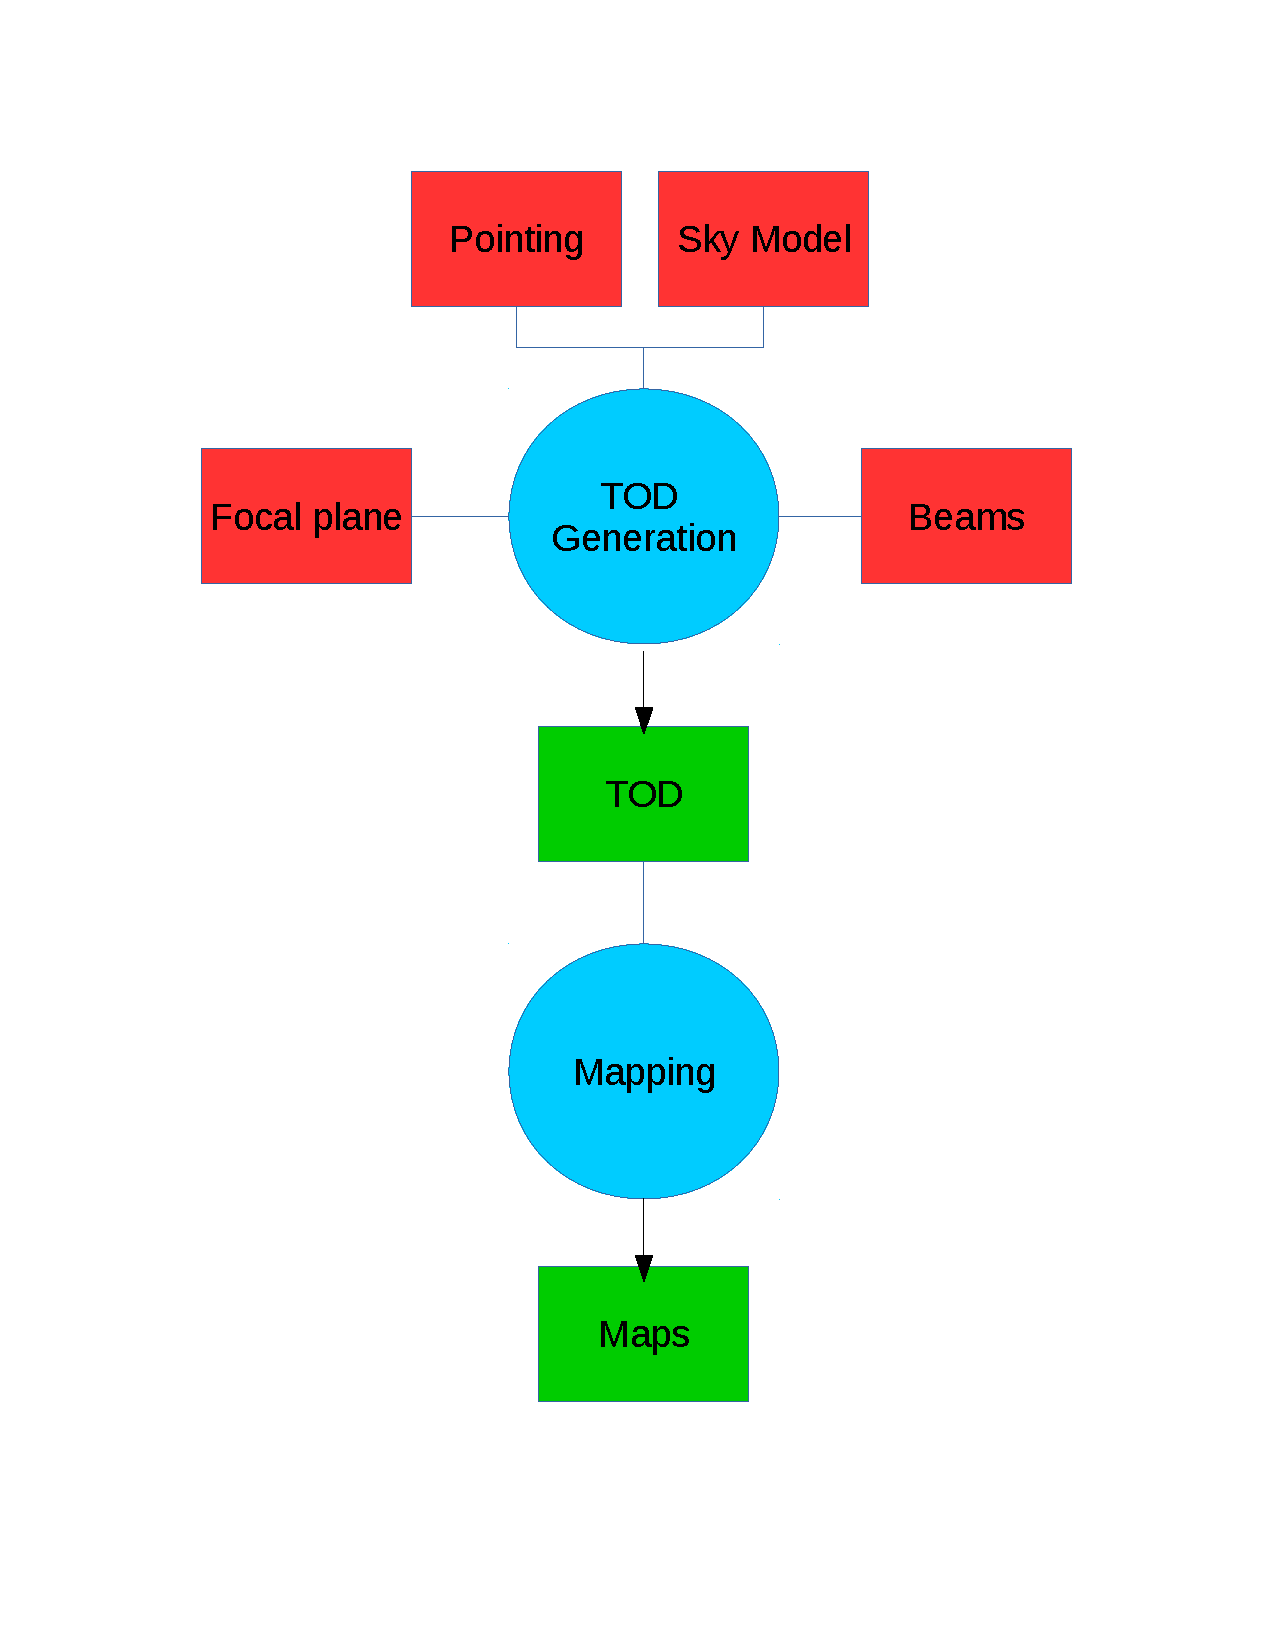
\includegraphics[width=0.6\linewidth]{figures/pisco-flow-diagram}
	\caption{Basic flow of a typical PISCO simulation pipeline. Red polygons show the required user input. PISCO uses this input and produces TOD (green polygon). This TOD stream is calculated using equation \ref{eq::discrete_beam_conv_tensor} for all pointing directions. TOD can then by sent into a mapper and, finally, to a power spectra estimator tool. PISCO does not compute pointing nor produces maps from TOD by itself; these tasks are left to external programs.}
	\label{fig::pisco_flow}
\end{figure}

\subsection{Implementation using CUDA}

\begin{figure}
	\begin{center}
		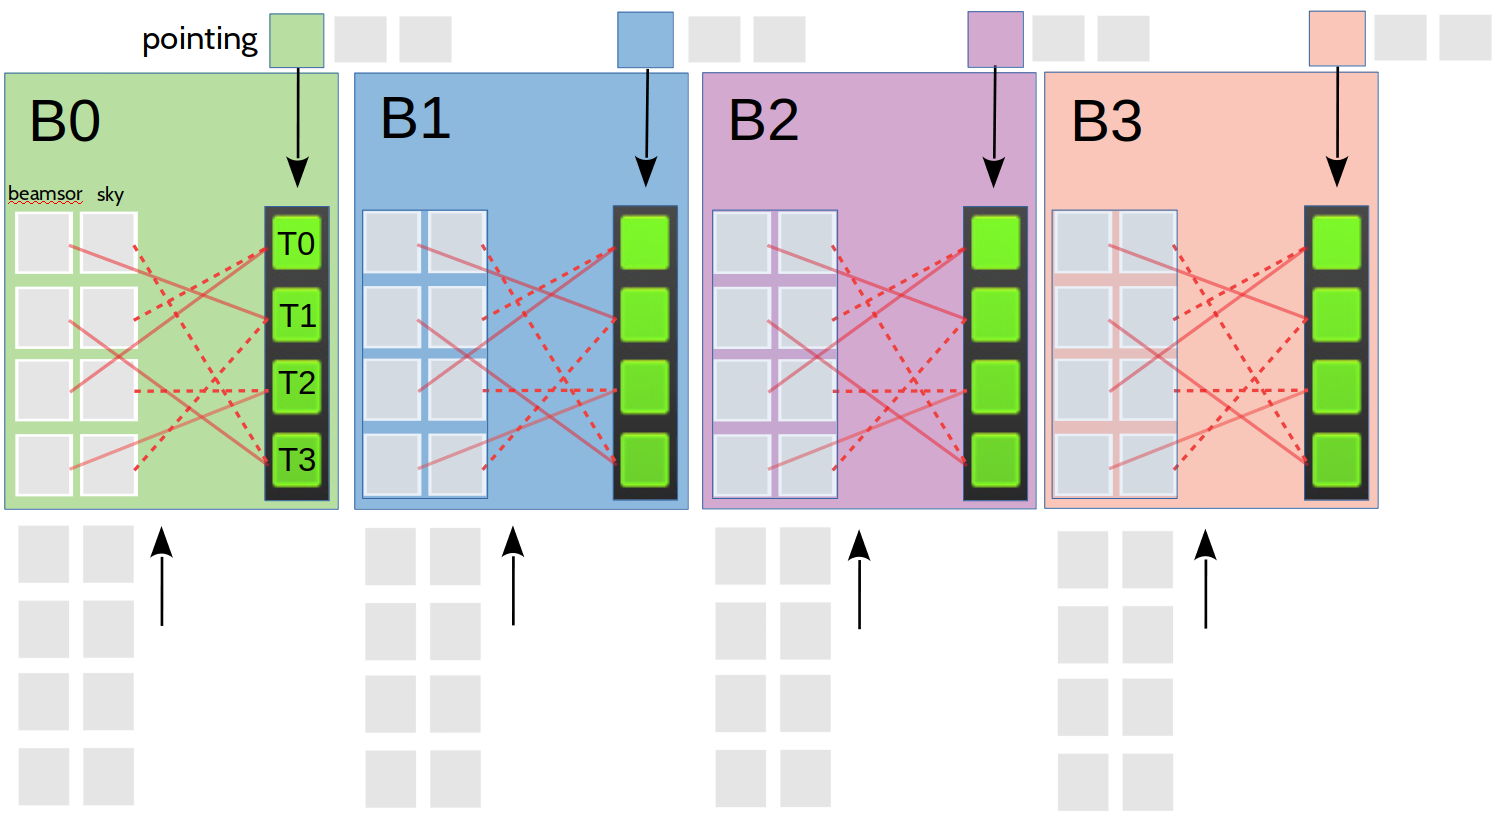
\includegraphics[width=0.8\linewidth]{figures/PISCO-diagram.png}
		\caption{Parallelization scheme. This figure shows the case of PISCO executing in 4 blocks ($B=4$), with four threads per block ($T=4$). Arrays with beamsor and sky elements are at the bottom. Each block has access to four beamsor and sky pixels (gray boxes inside colored boxes) and one pointing entry (colored small boxes) at a time. Green boxes represent the multiplication process of a single beamsor pixel with a single sky pixel. This includes rotating the sky pixel to the detector polarization basis, and computing the re-pixelization of $B$ at the corresponding coordinates. Solid and dotted red lines represent the complex memory access pattern generated by this process. Every thread within a block writes its result to shared memory space. When a thread finishes its computation, it waits until all threads have finished and a reduction on the shared memory space is performed across all blocks. This process is repeated for every pointing. At the end of the procedure, each block has computed the convolution of a beamsor with the sky for a particular pointing, and every shared memory space of the block has the corresponding result. These results are collected into the GPU global memory, which is then transferred back to CPU (host) memory.}
		\label{fig::pisco_diagram}
	\end{center}
\end{figure}

GPUs allow for substantial acceleration of algorithms that perform a large amount of independent operations. TOD generation using equation \ref{eq::discrete_beam_conv_tensor} presents an optimal application case because all operations are independent of each other. In this work, we used the Compute Unified Device Architecture framework from NVIDIA to implement the TOD generation routine. The reader is referred to \cite{sanders2010cuda} for an excellent description of CUDA and associated capabilities.

To better understand how the parallelism in \ref{eq::discrete_beam_conv_tensor} can exploited, consider the process of synthesizing $N_T$ measurements using a CUDA grid of $B$ blocks and $T$ threads. Consider each measurement to have an associated pointing $\bar{q}_t$ with $t=0..N_T$. PISCO performs a double parallelization scheme: the ``slow'' loop ($L1$) scans the pointing stream and associates every block to a pointing $\bar{q}_t$. A second, ``faster'' loop ($L2$), iterates over a list of pixels, which correspond to sky pixels that are ``inside'' the beamsor extension. This list of pixels is constructed in advance and then transferred to the GPU. $L2$ executes $T$ operations in parallel. Great care was taken to ensure no race conditions arise when multiple threads try to read (write) from (to) the same memory address. As every block executes $T$ convolution operations in parallel, and the CUDA grid runs $B$ simultaneous blocks, the parallelism is $B \times T$. Furthermore, if $G$ GPUs are available, the computation can be distributed among them, increases the parallelism to $G \times B \times T$. A graphical description of this process is shown in Figure \ref{fig::pisco_diagram}.

\subsection{Performance}

A simulation of a realistic CMB experiment (see Section \ref{sec::realistic_cmb_experiment} for more details) took approximately 45 minutes using a node equipped with two Intel Xeon E5-2610 processors (10 physical cores and 20 threads per processor), $256$ GB of RAM and one NVIDIA GTX 1080. This simulation generated 1 week of TOD, meaning that PISCO executed around 224 times faster than ``real time operation'' of the experiment. Unfortunately, measuring performance of the current implementation in FLOPS is a highly nontrivial task: the TOD generation routine performs both integer and floating point mathematical operations which are challenging to keep track of. In addition, we were not able to successfully quantify the impact of the memory access pattern caused by having to match beamsor pixels with sky pixels during the convolution step. Nevertheless, and in an effort to provide a comparison basis with other implementations, we report this simulation to have calculated more than $320000$ convolutions per second. It is quite possible for programs like \texttt{beamconv} (see \cite{2018arXiv180905034D}) to achieve much higher performance than PISCO for this particular test. It is worth noting, however, that PISCO has a small cost associated with increasing the complexity of the beam, i.e., by adding ghosting, high frequency features (in angular space) and time-dependent beam parameters, or transient events on the sky model, like varying temperature of the ground surrounding the receiver. This makes PISCO a good complement to other software tools that perform similar tasks because, while the computational cost might be larger for ``simpler'' cases (highly symmetrical beams and no time-dependent effects), the extra cost of adding another layer of complexity is comparatively low. %We also note that, to date, we are not aware of any other software tool that uses an equivalent formalism to beam tensors formalism explicitly.

\subsection{Future improvements}

The current implementation must calculate the list of sky pixels involved in each convolution, for all pointing directions, before the CUDA routine is launched. Having this list of pixels in memory decreases the available parallelism, as fewer pointing directions can be used at a given time. While the wall-time associated with this operation is modest, the result must be kept in memory and transferred to the GPU, so that the associated buffer quickly becomes too large to be held in the VRAM. Currently, PISCO handles this situation by performing the generation of TOD in blocks to avoid memory overflow. In the test machine, computing and transferring the lists of pixels can take up to $13\%$ of the \textsl{overall} simulation wall-time. A solution to this problem has already been devised and will be implemented in future releases. Another drawback of the current implementation is the use of global memory to hold the beam tensor elements. Future releases will exploit data locality by making use of the CUDA texture memory pipeline (see \cite{sanders2010cuda}). Finally, while the current implementation of PISCO was designed to execute in multiple GPU nodes, significant coding effort is required to provide the user with an easy to use interface. Experiments were performed emulating a multi-node system by making PISCO use all 3 GPUs of the machine. These tests showed an almost linear increase in performance, but more work is required in order to find the knee of the curve between performance and available GPUs.

%\begin{table}[tbp]
%	\centering
%	\begin{tabular}{|c|c|c|}
%		\hline
%		Routine description & Time (in seconds) & $\%$ of total time \\
%		\hline
%		convolution & 7967 & 52$\%$  \\
%		query pixel cap & 2171 & 14$\%$ \\
%		transfer pixel cap & 3978 & 27$\%$ \\
%		others & 985 & 7$\%$ \\ 
%		\hline
%	\end{tabular}
%	\caption{Table summarizing the times taken by different routines of PISCO. The simulation executed at more than 19 million convolutions per second.}\label{tbl1}
%\end{table}

% Sub-optimal performance might arise in the case of a slow storage device if a very large amount of pointing data is read from disc. Because of the way PISCO scales in multi-node systems, this situation should be greatly suppressed by using a parallel file-system, so as to exploit data locality and avoid expensive IO operations. We tested a worst case scenario where multiple GPUs read the pointing stream from a single Network Attached Storage (NAS) over a 1 Gigabit Ethernet connection. The pointing stream had more than 870 million individual directions and it was saved to disc as \texttt{NPZ} files. The data was read from the NAS using \texttt{numpy.load}. We found that the IO penalty was less than $5\%$ of the simulation wall-time. We note that this simulation did not write any TOD to disc.

%
\section{Code validation}
\label{sec::validation}

% This was already mentioned.
%All simulations were performed in a machine equipped with three NVIDIA GTX 1080 cards, two Intel Xeon E5-2610 processors (20 physical cores, 40 threads) and $256$ GB of RAM.  
To validate the correctness of PISCO, we performed two sets of tests: a mock observation of a (polarized) point source and a simulation of an ideal CMB observation. Results from these tests were compared against the \texttt{healpy.smoothing} routine, a Python wrapper around HEALPix routines, which calculates the convolution of a polarized sky with a circularly symmetric Gaussian beam in $a_{\ell m}$ space. For the purposes of this section, we will consider the output of \texttt{smoothing} to be exact. 

\subsection{Point source observations}

The simulated observation of a polarized point source was accomplished by the following steps

\begin{itemize}
    % Changing this to explicitly show the detectors and beams are ideal
    %\item Build a beamsor without cross-polarization Each $B_{ii}$ component is a circular Gaussian beam with FWHM of $1.5^\circ$.
    \item Build a beamsor with off-diagonal elements set to zero. Every $\tensor{B}{^i_i}$ element corresponds to a circular Gaussian beam with FWHM of $1.5^\circ$. 
    \item For simplicitly, we used a PSB with $s=1$ and $\epsilon=0$ for both detectors.
	\item Build a mock sky, with a single non-zero pixel at coordinates $(\theta_k,\phi_k)$. Three cases were run: unpolarized, pure Q polarization and pure U polarization.".
	\item Set up a raster scan around $(\theta_k,\phi_k)$ for a detector with $\zeta=0$. Note that, in order to have full polarization coverage, the raster scan is repeated 3 times with angles $\psi_0 = 0^{\circ},45^{\circ},90^{\circ}$.
	\item Make maps of TOD generated by PISCO.
	\item Compare the result of applying \texttt{smoothing} to the single pixel map using the same beam model.
\end{itemize}

\subsubsection{Results}

Results from this validation test are shown in Figure \ref{fig::stokesqsource256beam1024dec45}. The results show that the flux is preserved to better than $0.2\%$. For the \texttt{NSIDE} 256 sky used in this test, doubling \texttt{NSIDE} of the beam from 1024 to 2048 does not improve the preservation of the flux significantly (from $0.2$\% to $0.04$\%) at the cost of quadrupling the amount of memory required to store the beamsor, while using a lower \texttt{NSIDE} for the beam degrades this considerably to $0.8$\%. We conclude that a 4:1 beam to sky \texttt{NSIDE} ratio is sufficient. We also checked for systematic effects driven by the finite machine precision of the computations, and found that leakage from temperature to polarization was consistent with zero to machine precision. The maximum residual in the P to P leakage is on the order of $0.1\%$. PISCO is also able to correctly account for intra-beam variations of the position angle $\chi$.

\begin{figure}
	\centering
	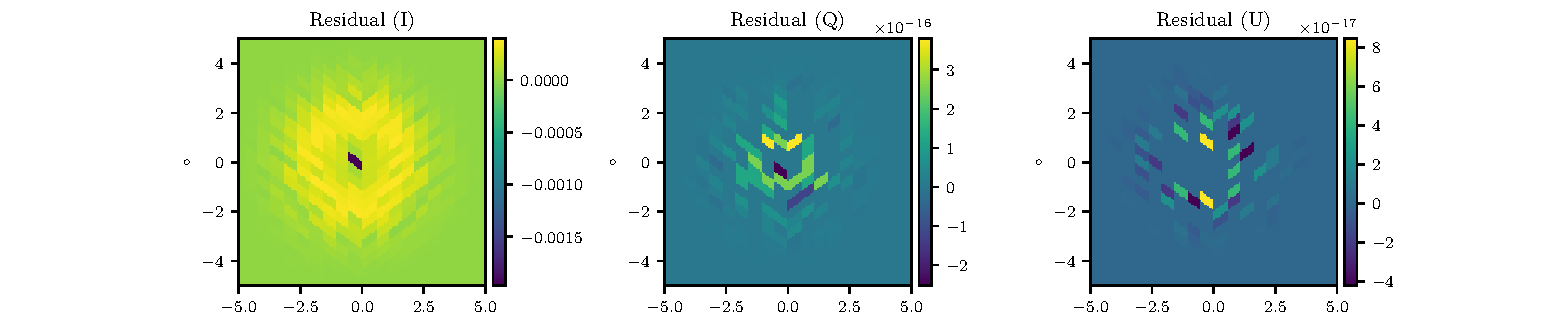
\includegraphics[width=1.0\linewidth]{figures/figure5_3rd_I.pdf}
	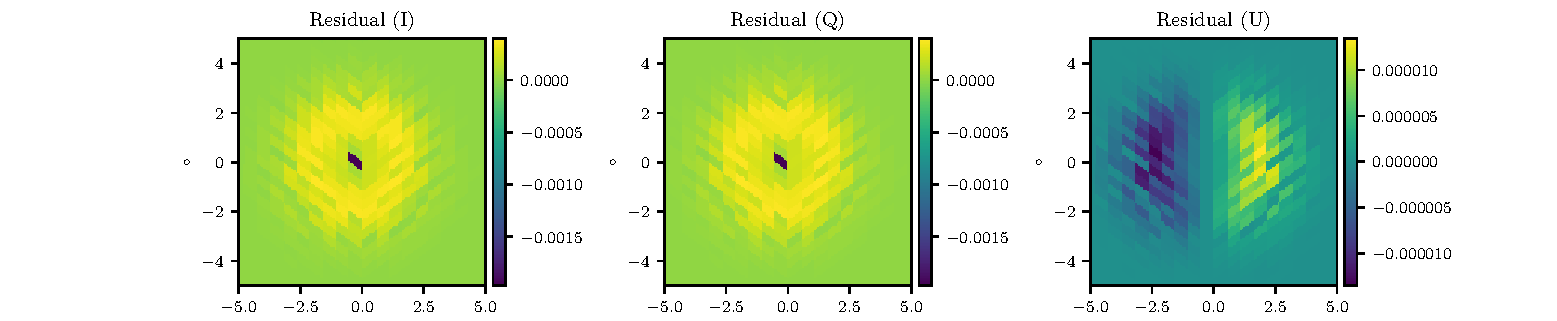
\includegraphics[width=1.0\linewidth]{figures/figure5_3rd_Q.pdf}
	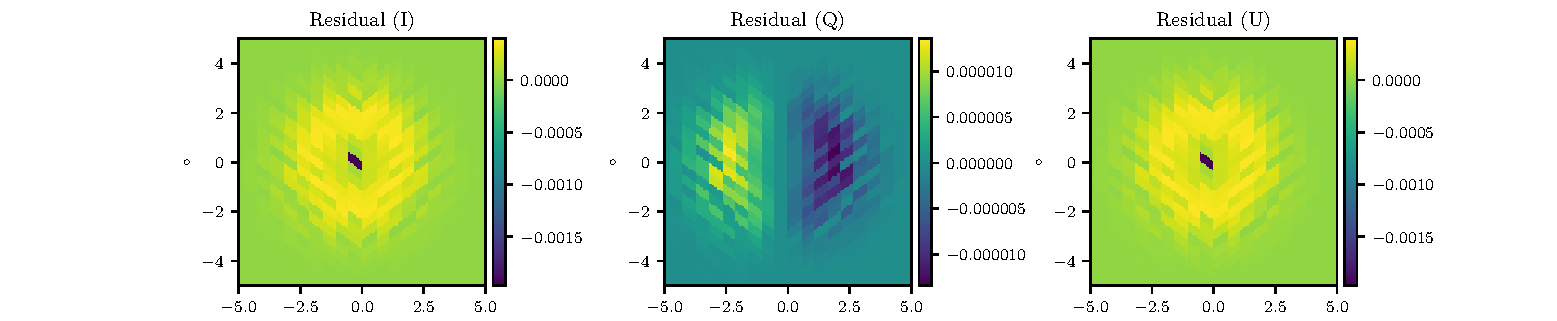
\includegraphics[width=1.0\linewidth]{figures/figure5_3rd_U.pdf}
	\caption{Plots showing the result of differencing a map with a point source convolved with a Gaussian beam using \texttt{smoothing} and the map generated from PISCO TOD. The input map used HEALPix pixelization with $\mathrm{\texttt{NSIDE}} = 256$, while the beamsor resolution was set to $\mathrm{\texttt{NSIDE}} = 1024$. The Gaussian profile used for the beamsor had a FWHM of $1.5^\circ$. All point sources were located at $45^\circ$ declination. The color scale is normalized to $1$,which is also the amplitude of the source. From top to bottom: residuals for the case of a point source with Stokes vector $S = (1,0,0,0)$, $S=(1,1,0,0)$ and $S=(1,0,1,0)$, respectively.}
	\label{fig::stokesqsource256beam1024dec45}
\end{figure}

\subsection{Ideal CMB experiment}
\label{subsec::ideal_full_sky}

\subsubsection{Description}

%As in the point source case, the simulation of an ideal CMB experiment was accomplished by the following:
The simulation of an ideal CMB experiment was accomplished by the following:

\begin{itemize}
    %\item Build a beamsor without cross-polarization Each $B_{ii}$ component is a circular Gaussian beam with FWHM of $1.5^\circ$.
    % I adding this to explictly say detectors are perfect
    \item Build a beamsor with off-diagonal elements set to zero. Every $\tensor{B}{^i_i}$ element corresponds to a circular Gaussian beam with FWHM of $1.5^\circ$. 
    \item For simplicitly, we used a PSB with $s=1$ and $\epsilon=0$ for both detectors.
    \item Build mock CMB whole sky maps with a tensor-to-scalar ratio $r=0.0$.
	\item Set up a scanning strategy to visit each pixel center at 3 different position angles $\psi_0 = 0^{\circ},45^{\circ},90^{\circ}$. 
	\item Make maps of TOD generated by PISCO. 
	\item Compare spectra generated from the maps with spectra of the input maps.
\end{itemize}

\subsubsection{Sky model}
\label{subsec::sky_model}

The input sky maps were generated using a combination of CAMB (see \cite{Lewis:2002ah}) to generate $C_\ell$, and \texttt{synfast} to generate maps from the $C_\ell$. The cosmological parameters are consistent with those reported by the \textsl{Planck} satellite collaboration (see \cite{2016A&A...594A..13P}). This procedure returns 3 CMB anisotropy maps, one for each Stokes parameter. The CMB is not expected to have Stokes $V$ polarization, so this field was explicitly set to zero. CAMB was configured to return a CMB with no primordial B-modes ($r=0$) and no lensing, as this last effect is expected to transform E-modes to B-modes. The resulting B-mode power spectrum is effectively zero at all angular scales. No foreground or other sources were added on top of the simulated CMB. All maps use the \texttt{HEALPix} pixelization and were generated at a resolution of \texttt{NSIDE}$=128$. This restricts the analysis in harmonic space to $\ell < 384$.

\subsubsection{Scanning strategy}

The scanning strategy was designed so that every pixel on the sky gets visited exactly three times, each time at a different beam orientation angle. In addition, every pixel was observed at its center, which is an important requirement that ensures the intra-pixel coverage does not affect the estimation of the power spectra at high $\ell$. Since only three hits per pixel at different values of $\chi$ are required to recover the polarization field of the CMB, the scanning was generated for a single detector with a polarization sensitive angle $\zeta=0$.

\subsubsection{Power spectra}

Power spectra were calculated using \texttt{anafast}. No further post-processing of the power spectra was needed given that this simulated observation covers the whole sky, and hence no masking effects arise. The power spectra corresponding to maps that were generated using PISCO TOD were corrected by dividing by the equivalent beam transfer function of a circular Gaussian beam of FWHM $1.5^\circ$. 

\subsubsection{Results}

\begin{figure}
	\centering
	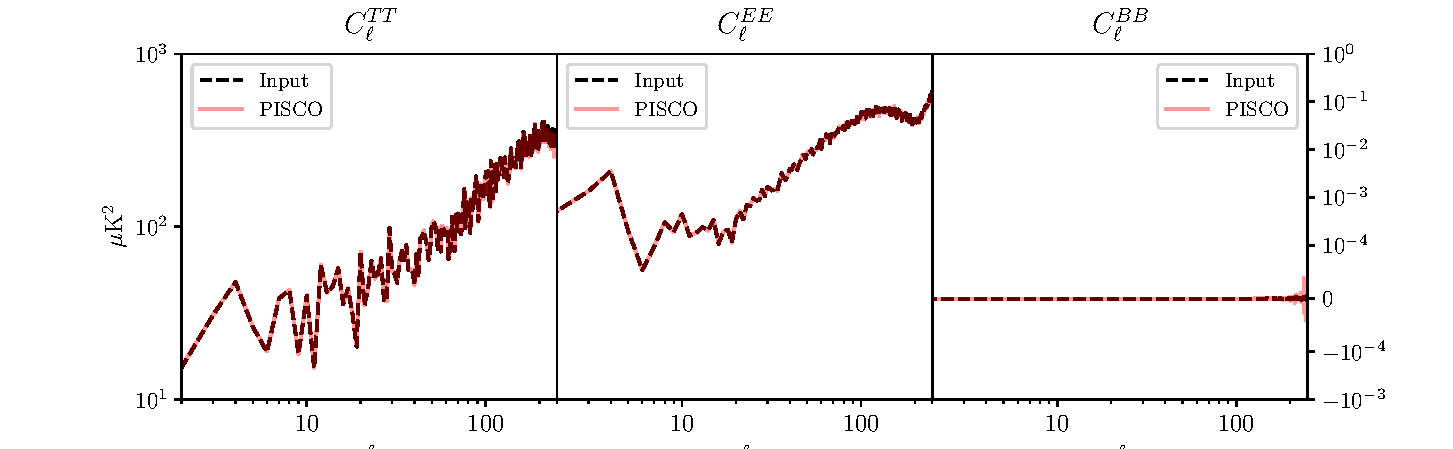
\includegraphics[width=1\linewidth]{figures/cmb_r0d00_CLASS_wholeskytest.pdf}
	\caption{Plot showing spectra from PISCO generated TOD (red, solid curve) for the whole sky CMB test (black, dashed curve). Excellent agreement is observed, with no leakage from E-modes to B-modes or from temperature to polarization. }
	\label{fig::pisco4wholesky}
\end{figure}

The main result of this simulation is shown in Figure \ref{fig::pisco4wholesky}. A single simulation took less than 100 seconds on the testing machine. We report no indications of leakage from temperature to polarization, nor from E-modes to B-modes. It is worth noting that this process was repeated using several realizations of roughly the same cosmology, but with varying values of $r$. We found no evidence of leakage in any of these cases. There is an oscillatory behavior around $\ell=250$ in the case of $BB$. This can be explained by the effect of the beam transfer function, which has large impact at those angular frequencies, and thus makes the estimation of the power spectra uncertain. Repeating this experiment using a beam with smaller $\rm{FWHM} = 1.0^{\circ}$ shifted this discrepancy to higher $\ell$, indicating that this hypothesis is valid. 

% Chaging this to "CMB experiment with realistic scanning strategy"
%\section{Realistic CMB experiment}
\section{A more realistic CMB experiment}
\label{sec::realistic_cmb_experiment}

% After some ping-pong with MKB, this is was changed to the what's below.
%The tests performed in Section \ref{subsec::ideal_full_sky} correspond to an idealized case. In this section, we show results for a simple, but more realistic, application of PISCO. The focus of this section is to demonstrate that the implementation of the model presented in Section \ref{sec::antennas} is able to reproduce the effects of pointing and beam mismatch, which that can cause T to P leakage (see \cite{Ade_2019ywi}), and uneven intra-pixel coverage, which can cause divergence in the polarization power spectra at high $\ell$ (see \cite{2005poutanen}). We did not include other systematic effects like gain imbalance, detector efficiency, cross-polarization responses and far sidelobes. 

The tests performed in Section \ref{subsec::ideal_full_sky} correspond to an idealized case. In this section, we show results for a simple, but more realistic, application of PISCO. The focus of this section is on demonstrating that the implementation of the model presented in Sections \ref{sec::antennas} and \ref{sec::pisco} is able to reproduce the expected effect of pointing and beam mismatch, which is T to P leakage (see \cite{2007MNRAS.376.1767O}), and uneven intra-pixel coverage, which is P to P leakage (see \cite{2005poutanen}). As in the previous section, we did not include other systematic effects like gain imbalance, detector efficiency, cross-polarization responses and far sidelobes.
 
\subsection{Description of the simulations}

Since designing such an experiment from scratch is a challenging task, we turned to simulating an ongoing mission, the Cosmology Large Angular Scale Surveyor, CLASS. CLASS aims at characterizing the CMB anisotropy field at large angular scales, particularly the power spectra of B-modes and E-modes, looking for evidence of inflation. While the experiment is composed of 4 telescopes, the simulation focuses on the one observing at the lowest frequency (38 GHz), the Q-band receiver, which has a 1.5 degree beam. This decision was taken for computational reasons, mainly because Q-band has lower detector count compared to higher frequency receivers. We note that CLASS uses modulation techniques to increase its sensitivity to CMB polarization. The effects of modulation related systematics have been described elsewhere (\cite{2016ApJ...818..151M}). For a more detailed description of CLASS, the reader is referred to \cite{2016SPIE.9914E..1KH}, \cite{2014SPIE.9153E..1IE} and \cite{2019ApJ...876..126A}.

\subsubsection{Sky model}

To generate the maps for this simulation, we followed a similar procedure to the one described in section \ref{subsec::sky_model}. The main difference is the addition of a temperature only CMB, which was used to check for T to P leakage caused by effects that were not present in the last test presented in Section \ref{sec::validation} All maps use the \texttt{HEALPix} pixelization with an \texttt{NSIDE} parameter of $128$. 

\subsubsection{Pointing}

The scanning strategy of CLASS consists of constant elevation scans (CES). Elevation is kept at $45^{\circ}$ while the telescope rotates $720^\circ$ in azimuth at $1$ degree per second. Under normal survey conditions, the telescopes scan nearly 24 hours a day. The boresight is rotated from $-45^{\circ}$ to $+45^{\circ}$ by $15^{\circ}$ per day on a weekly schedule. This scanning strategy, in combination with the large CLASS field of view results in the telescopes covering more than 70$\%$ of the sky. In addition, because of the boresight rotation, only seven days are needed to provide excellent position angle coverage. While CLASS records data $200$ times per second, the pointing streams were generated at $20$ Hz. Down-sampling by a factor of 10 results in a ten-fold decrease in computation time with the median number of hits per pixel still being on the order of thousands. Even with this significant reduction, the pointing stream contained more than 870 million samples.

%Taking into account the above considerations, the boresight pointing was generated by closely emulating the scanning strategy in horizontal coordinates (constant elevation scans). Next, 
%The equatorial coordinates for every detector on the focal plane were calculated using this stream and the beam center offsets of the detector. We note that this procedure does not take into account telescope down-time caused by daily maintenance or other systematic effects, like variations in the pointing model. The scanning strategy that was used for this simulation corresponds to seven continuous streams of 24 hours, one for each boresight angle, sampled at $20$ Hz. The pointing stream has more than 870 million individual pointing directions. 

Equatorial coordinates of every detector were computed from the horizontal coordinates produced by the scanning strategy and the beam center offsets of every detector from the center of the array.
Representative beam center offsets for the Q-band receiver were provided by the CLASS collaboration. Two streams were generated by considering detector pairs to have matched or mismatched offsets. The case of matched offsets was simulated by forcing each pair to share the same beam center offsets, which in turn were calculated as the average of the individual pair offsets. %Treating the deviation of every offset with respect to the pair average as a Gaussian random error yields an root mean squared mismatch of approximately $5$ arc-seconds ($\approx 0.001^{\circ}$).

\subsubsection{Beamsor model}

%Following the work of \cite{2012SPIE.8452E..20E} and input from the CLASS collaboration, we built beamsor models for all 72 detectors of the Q-band. The two dimensional profile of the diagonal beamsor elements correspond to purely elliptical Gaussian profiles, while the off-diagonal terms were set to zero.

%We calculated the degree of beam mismatch from beam parameters following a similar procedure as for the beam center offsets. The root mean square mismatch for $\rm{FWHM}_x$ and $\rm{FWHM}_y$ is $0.01^{\circ}$.
%The CLASS collaboration also provided us with representative main beam parameters. The main beam parameters correspond to FWHM in the East-West direction ($\rm{FWHM}_x$), FWHM in the North-South direction ($\rm{FWHM}_y$) and the rotation angle of the major axis of the corresponding elliptical profile. Q-band receiver was designed to observe the sky with a Gaussian beam of FWHM=$1.5^\circ$. The simplicity of the beams allows a further speed-up in the computation by restricting the convolution to a $5^\circ$ disc around the beam center. This value was chosen as because a pixel that is $5^\circ$ away from the centroid of the beam has a value of $\approx 10^{-14}$, roughly the limit of double precision arithmetic. All beamsors were pixelated using $\rm{NSIDE}=512$. The finite resolution of the beamsor produces an error in the amplitude of simulated TOD that is less than $0.1\%$ compared to analytical estimations, which is consistent with the results described in Section \S\ref{sec::validation}.

The CLASS collaboration also provided us with representative main beam parameters. The main beam parameters correspond to FWHM in the East-West direction ($\rm{FWHM}_x$), FWHM in the North-South direction ($\rm{FWHM}_y$) and the rotation angle of the major axis of the corresponding elliptical profile. The simplicity of the beams allows a further speed-up in the computation by restricting the convolution to a $5^\circ$ disc around the beam center. This value was chosen as, for a unit normalized Gaussian beam, a pixel that is $5^\circ$ away from the centroid of the $1.5^{\circ}$ FWHM beam of the CLASS Q band receiver has a value of $\approx 10^{-14}$, roughly the limit of double precision arithmetic. All beamsors were pixelated using $\rm{NSIDE}=512$. The finite resolution of the beamsor produces an error in the amplitude of simulated TOD that is less than $0.1\%$ compared to analytical estimations, which is consistent with the results described in Section \S\ref{sec::validation}.

%\begin{figure}
%	\centering
%	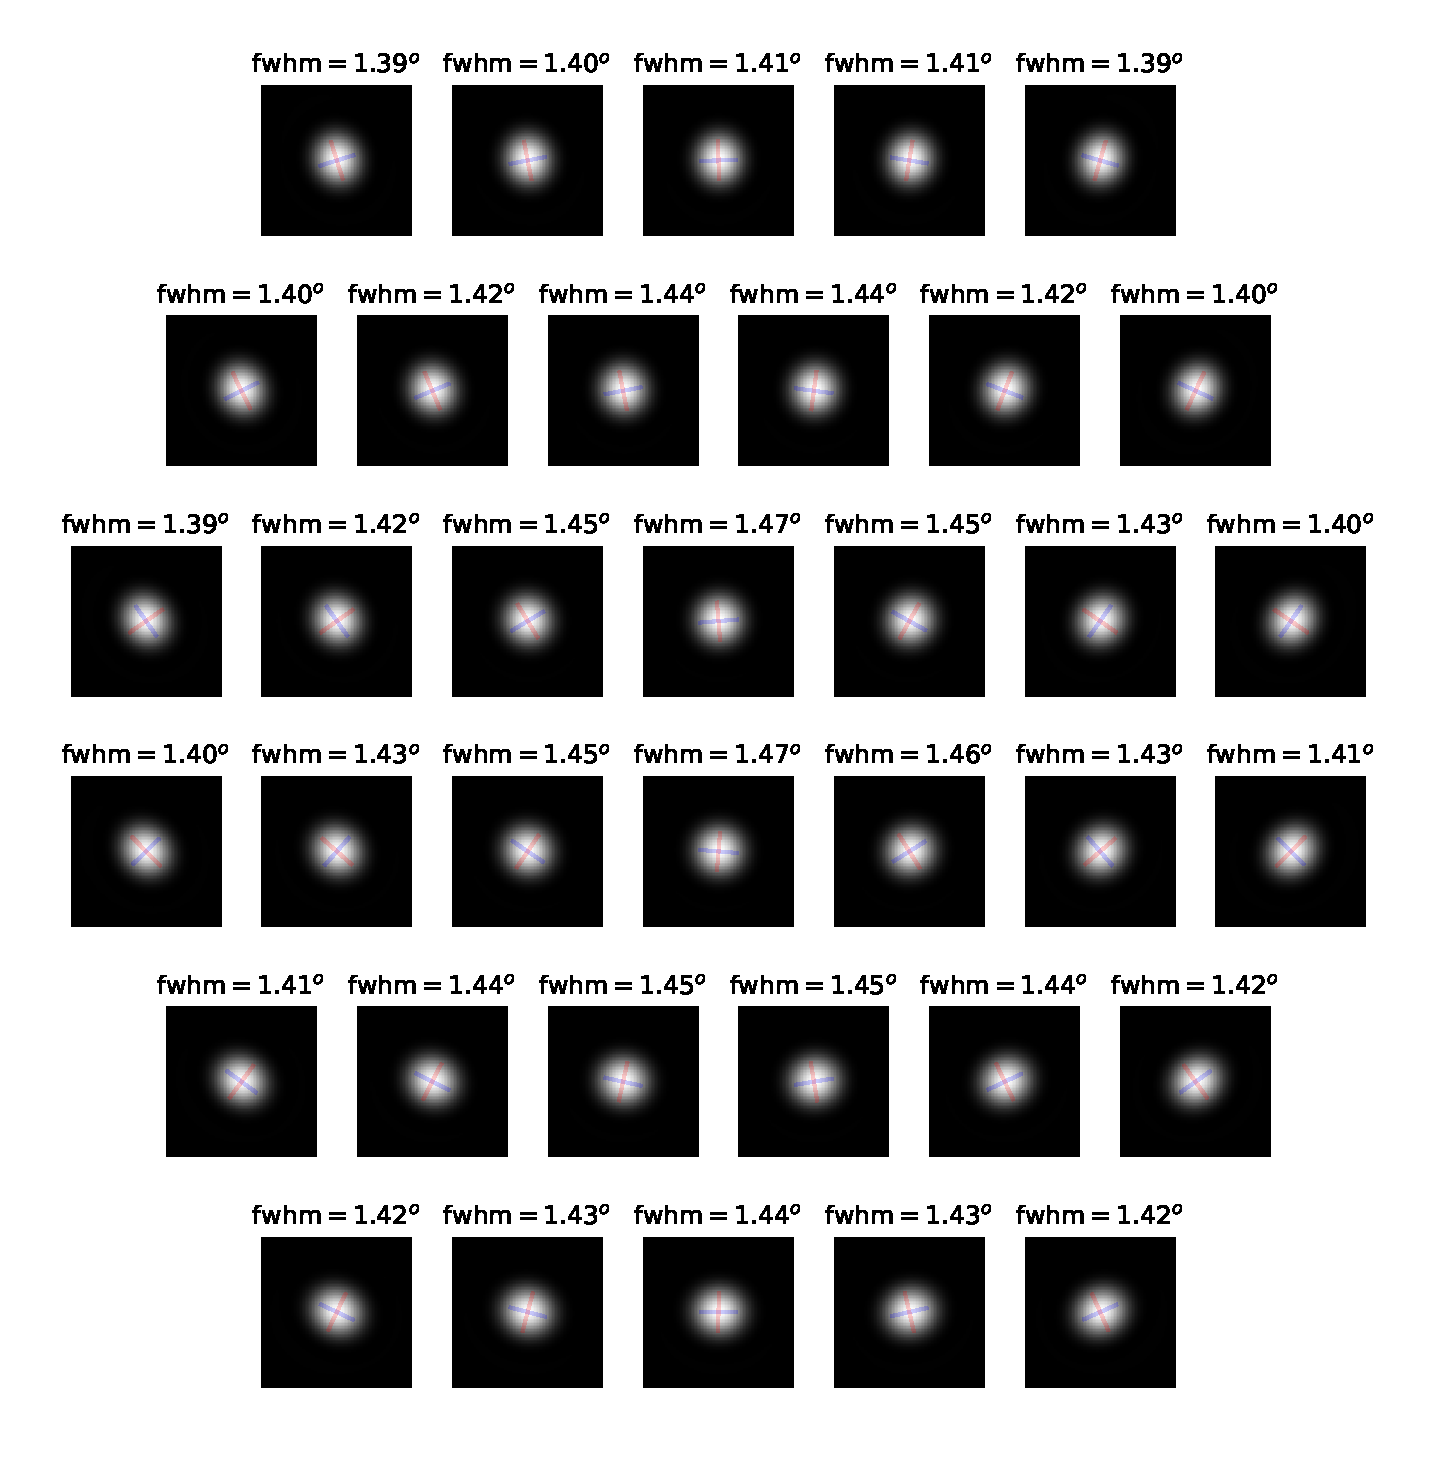
\includegraphics[width=0.8 \linewidth]{figures/qband_beams_main_beam_fwhm_x}
%	\caption{Elliptical Gaussian profiles used as beamsor models for the CLASS Q-band telescope. Relative positions of plots are representative of the positions of feedhorns on the sky. In image coordinates, Zenith is up while East is to the left. All beam profiles are unit normalized, the color scale being linear. Each subplot is a plane projection on the sky of $5^\circ \times 5^\circ$. The title of each subplot is the Full Width at Half Maximum of the profile along its semi-major axis. Non negligible amounts of eccentricity can be seen in the beam profiles, and a visible correlation between beam location on the sky, beam eccentricity and orientation of the major (minor) axis is present. Maximum eccentricity reaches $0.45$ for edge beams.}
%	\label{fig::qbandbeamsmainbeamfwhmx}
%\end{figure}

\subsubsection{Power spectra and beam transfer function}

Given that CLASS only covers $\approx 70\%$ of the sky, computing the power spectra of simulated maps requires the use of a tool than can handle a sky mask. For this reason, we changed the estimator from \texttt{anafast} to \texttt{Spice} through the \texttt{PolSpice} implementation (see \cite{2004MNRAS.350..914C}). In addition, the CLASS collaboration provided a realistic sky mask that includes the galactic plane as well as the sky outside the survey boundaries.

While the effect that smooth, circularly symmetric beams have on the power spectra is known (see \cite{2003ApJS..148...39P}), beams for CLASS have non-zero eccentricity and so we need to account for the effect of this on the CMB power spectra. This is done by computing the radial profile of each beam through an analytical integration over $\phi$, averaging the radial profiles of all of the beams in the array receiver and then calculating the harmonic transform of the average profile to use as the beam transfer function in deconvolving the power spectra.

%While the effect that smooth, circularly symmetric beams have on the power spectra is known (see \cite{2003ApJS..148...39P}), beams for CLASS have non zero eccentricity and so we need to account for the effect of this on the CMB power spectra. We chose to symmetrize the beams and then estimate the equivalent beam transfer function by averaging the radial profiles, which in turn were obtained from an analytical integration over $\phi$ of all of the beams in ``real'' space. We then calculated the harmonic transform of the average profile and corrected for it in power spectra space.

%Given that, at present, CLASS only covers $\approx 75\%$ of the sky, computing the power spectra of simulated maps requires the use of a tool than can handle a sky mask. For this reason, we changed the estimator from \texttt{anafast} to \texttt{Spice} though the \texttt{PolSpice} implementation (see \cite{2004MNRAS.350..914C}). In addition, the CLASS collaboration provided a realistic sky mask that includes the galactic plane as well as the natural incomplete coverage. 
%In addition, we need to account for the effect of the beam on the CMB power spectra. This can be thought of as a low-pass filter in harmonic space (see \cite{2003ApJS..148...39P}). We estimated the equivalent beam transfer function of an arbitrary number of elliptical beams by averaging the radial profiles obtained from an analytical integration over $\phi$ of all of the beams in ``real'' space,  and calculating the harmonic transform of the average profile.

\subsubsection{A unified metric for describing mismatch }
\label{sec::mismatch_metric}

While it is simple to use the difference in pointing between two paired detectors to describe pointing mismatch, elliptical beam mismatch involves three quantities: the difference in the semi-major beam widths, the difference in the semi-minor beam widths and the difference in orientation of the two elliptical beams on the sky. When multiple pairs are considered, it becomes unclear how to average these parameters in order to gain insight into the degree of mismatch in the set. For this reason, it is desirable to define a metric that can be suitably applied to more than one pair. One such metric can be derived from the difference $\Delta b(\rho,\sigma)$ in the fitted elliptical Gaussian beams for the detector pair of each PSB by considering the maximum difference expressed as a percentage of the normalized beams, namely

\begin{equation}
\delta_{(p,b)} = \rm{max}\left| \Delta \mathit{b}_{(p,b)}(\rho,\sigma) \right|
\end{equation}

\noindent
where the subscripts $p$ and $b$ represent the cases of pointing mismatch and beam mismatch respectively (see Figure \ref{fig::mismatch_metric}). This unified metric is directly proportional to the difference in convolution weighting for each detector pair and can be meaningfully averaged over multiple pairs. 

\begin{figure}
	\centering
	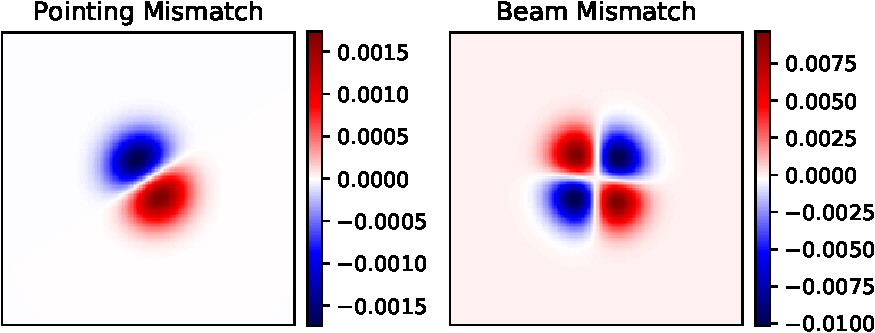
\includegraphics[width=0.7\textwidth]{figures/PairDiffSinglePair-crop.pdf}
	\caption{Example pair differenced elliptical Gaussian beams for pointing mismatch and beam mismatch. The resulting metrics are $\delta_p = 0.17\%$ and $\delta_b = 1.0\%$.}
	\label{fig::mismatch_metric}
\end{figure}

\subsection{Results and discussion}

\subsubsection{Matched pointing and beams}

For the purpose of comparison, a test was run using matched beams. This was done by averaging both the pointing offsets and elliptical beam parameters for each detector pair in the array. The results of this test are shown in the upper plot of Figure \ref{fig::pisco4class_pointingmismatch}. In this and all subsequent plots the theoretical E-mode and B-mode spectra for a universe with $r=0.01$ were overlaid to provide context. As expected, the result of this test is that there is no T to P leakage present.   


\subsubsection{Pointing mismatch}

CMB experiments that rely on detector pairs are subject to leakage caused by pointing mismatch. As described in the work of \cite{2007MNRAS.376.1767O}, differential pointing between individual detectors belonging to the same PSB couples to gradients in the temperature field.

This test was performed by using the pointing offsets of the individual detectors while averaging the elliptical beam parameters for each detector pair in the array. Applying the metric described in \S\ref{sec::mismatch_metric} to the beams used in this simulation yielded an average value of $\delta_p = 0.42\%$ for the resulting pair differenced pointing mismatch. 

The leakage caused as a result of this pointing mismatch is presented in the lower plot of Figure \ref{fig::pisco4class_pointingmismatch}. We found that the spurious B-mode signal produced by pointing mismatch reaches $10 \, \rm{pK}^2$ at $\ell=100$, rising to $30 \, \rm{nK}^2$ at $\ell=250$. In contrast, the amplitude of the theoretical B-mode power spectrum for $r=0.01$ reaches $\approx 40 \, \rm{pK}^2$ at $\ell=100$. The leakage driven B-mode spectrum becomes dominant after $\ell=120$.

%Leakage arises at the map-making stage and is caused by an incomplete cancellation of the Stokes $I$ term when solving for the individual pixel-covariance matrices. This residual term from the Stokes $I$ is interpreted by the map-making algorithm as a polarized signal, hence causing the leakage shown in figure \ref{fig::pisco4class_pointingmismatch}. %We note that leakage is not present below $\ell \approx 100$, but becomes dominant at increasing angular frequencies. We believe this is caused by the effect of pointing mismatch being restricted to angular scales comparable to the FWHM of the beam. 

\begin{figure}
    \centering
    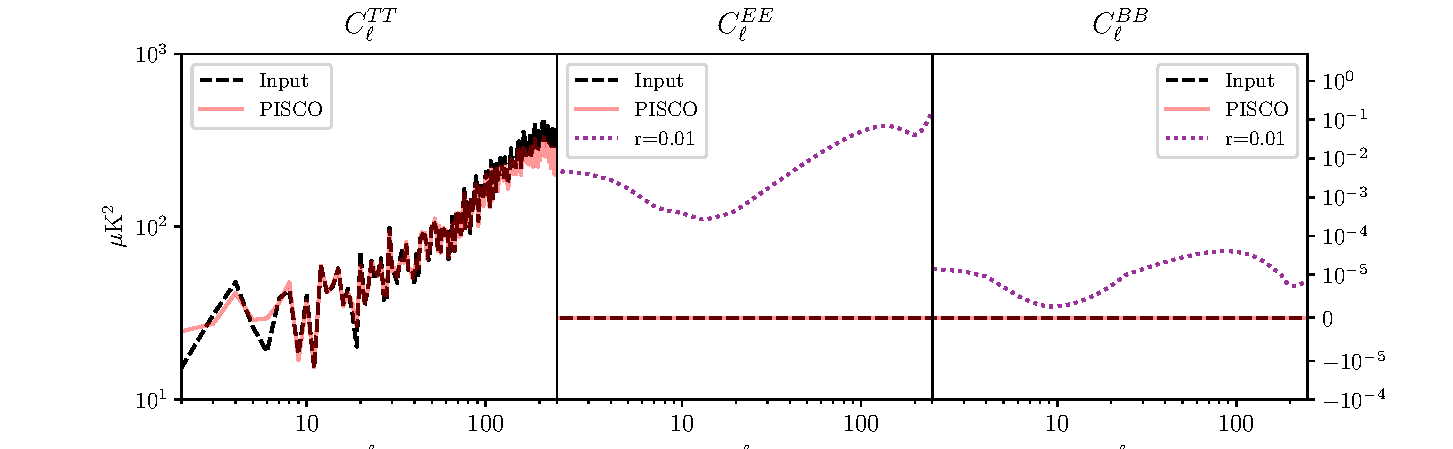
\includegraphics[width=1\textwidth]{figures/unpol.pdf}
    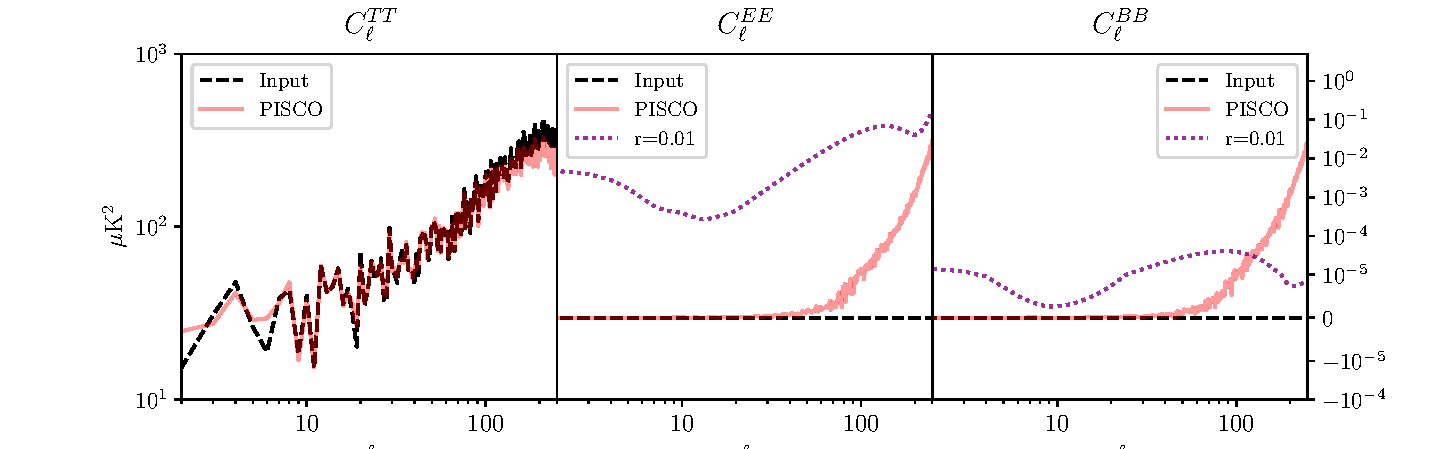
\includegraphics[width=1\textwidth]{figures/pointingMismatch.pdf}
	\caption{Resulting power spectra for a realistic simulation using matched pointing (upper figure), and mismatched pointing (bottom figure). The input CMB was unpolarized. Leakage from $TT$ to $EE$ and $BB$ power spectra is present for the mismatched pointing simulation. Reference E-mode and B-mode power spectra for a CMB with $r=0.01$ are shown using the purple, dashed line. The spurious signal reaches $30\, \rm{nK}^2$ at $\ell = 250$, for both $EE$ and $BB$.}
	\label{fig::pisco4class_pointingmismatch}
\end{figure}

\subsubsection{Beam mismatch}

\begin{figure}
	\centering
	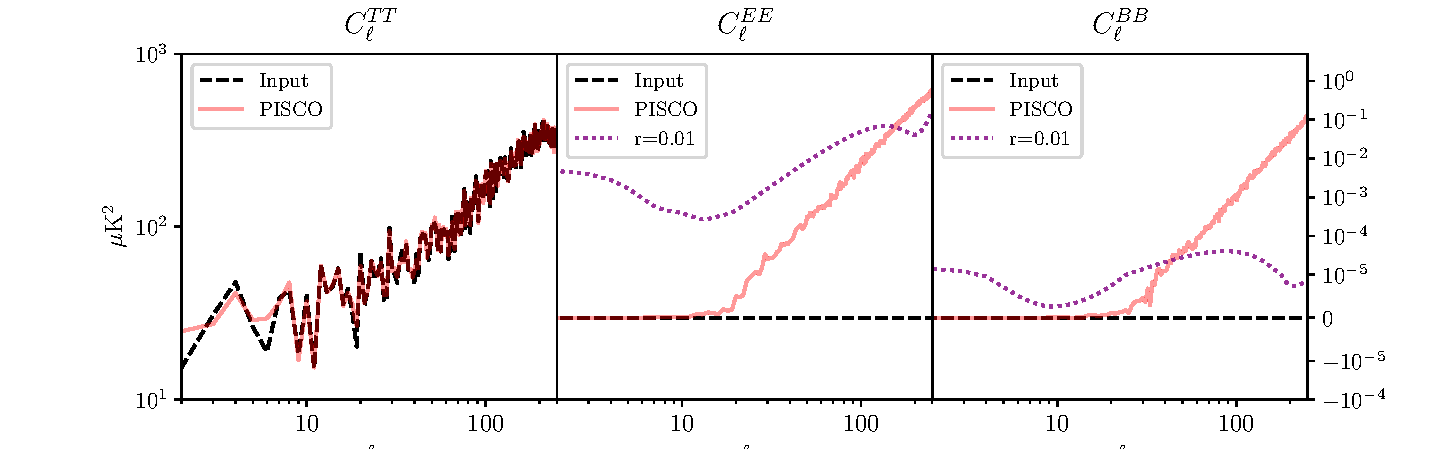
\includegraphics[width=1\textwidth]{figures/beamMismatch.pdf}
	\caption{Resulting power spectra of a realistic simulation from which the effects of uneven intra-pixel and pointing mismatch have been suppressed. The input CMB was unpolarized, so that the resulting E-mode and B-mode power spectra can only be a result of T to P leakage. Reference E-mode and B-mode power spectra for a CMB with $r=0.01$ are shown using the purple, dashed line. The amplitude of the leakage signal reaches roughly $0.1\, \mu\rm{K}^2$ at $\ell=250$, and dominates over a B-mode power spectrum (for $r=0.01$) above $\ell=42$.}
	\label{fig::pisco4class_beammismatch}
\end{figure}

Beam mismatch produces leakage from temperature to polarization by introducing a coupling between the beam and local quadropole-like patterns in the temperature fields (see \cite{2007MNRAS.376.1767O}) 

This test was performed by using the elliptical beam parameters of the individual detectors while averaging the pointing offsets for each detector pair in the array. Applying the metric described in \S\ref{sec::mismatch_metric} to the beams used in this simulation yielded an average value of  $\delta_b = 1.73\%$ for the resulting pair differenced beam mismatch. 

Figure \ref{fig::pisco4class_beammismatch} shows the resulting power spectra. The leakage reaches around $1\, \rm{nK}^2$ at $\ell=100$, rising up to $100 \, \rm{nK}^2$ at $\ell=250$. The spurious B-mode signal becomes dominant when compared to the theoretical spectrum of primordial B-modes for $r=0.01$ after $\ell=42$. We note that leakage also becomes dominant with respect to the E-mode power spectrum above $\ell=150$. 

\subsubsection{Uneven intra-pixel coverage}

Simulating a CMB experiment using a more realistic scanning strategy can produce another systematic effect at the power spectra level. This source of noise is related to the intra-pixel coverage of the sky. In section \ref{subsec::ideal_full_sky}, all pixels were observed exactly at their centers while, in a real experiment, every sample of the TOD ``hits'' a given pixel at an arbitrary location within it. If the distribution of hits inside a pixel is symmetric with respect to pixel center coordinates, map-making will average all observations and the power spectra from the resulting map will not be affected. However, if this distribution is asymmetric and gradients between pixels are present (recall that pixel space convolution is affected by neighbor pixels) the resulting power spectra may suffer from P to P leakage. This was discussed in more detail in \cite{2005poutanen}. 

\begin{figure}
	\centering
	%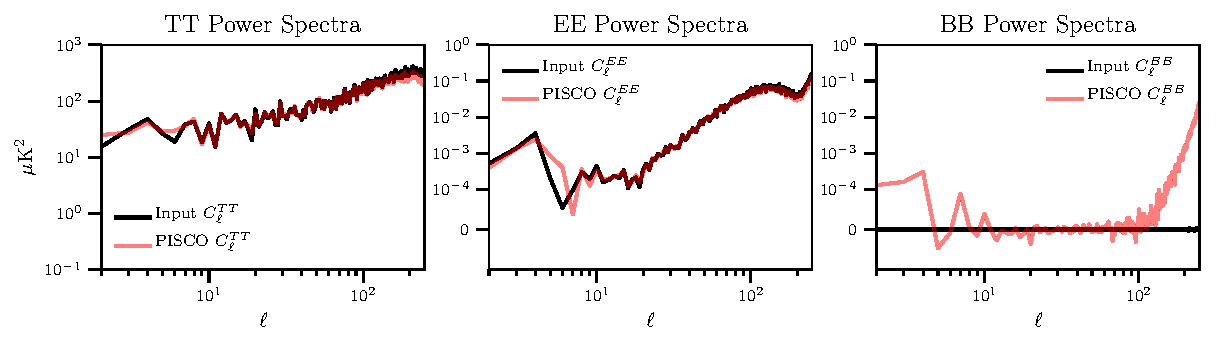
\includegraphics[width=1\textwidth]{figures/cmb_r0d00_CLASS_mismatchedPointing_matchedBeams_ellipticalBeams.pdf}
	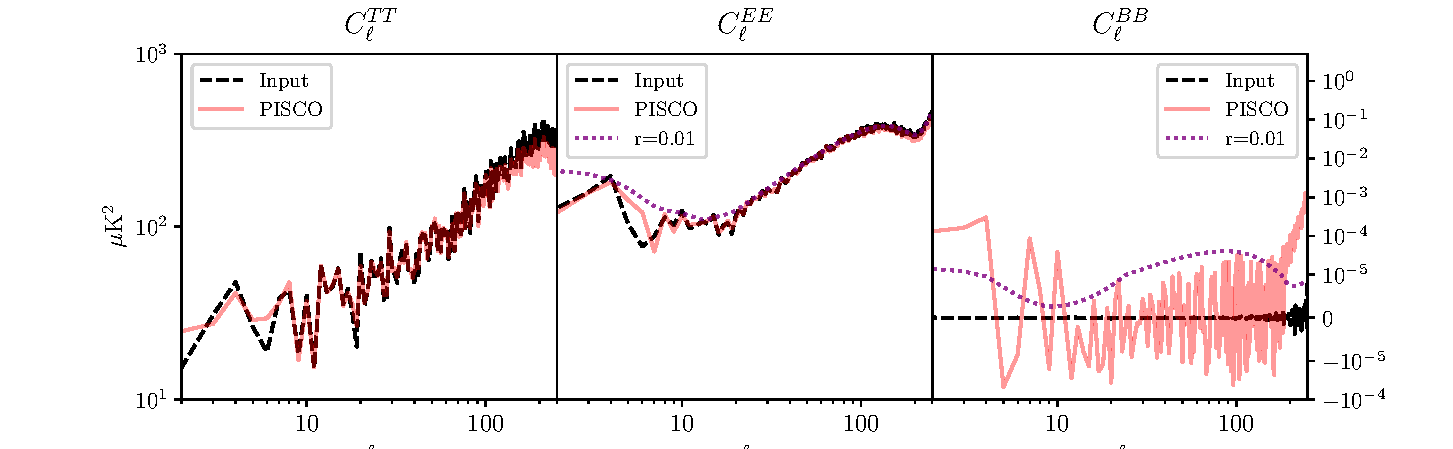
\includegraphics[width=1\textwidth]{figures/intrapixel.pdf}
	\caption{Resulting power spectra for the case of matched pointing with uneven intra-pixel coverage using as input a polarized CMB without B-modes. The B-mode power spectrum shows non-negligible amounts of a spurious signal not present in the input power B-mode power spectrum. Reference E-mode and B-mode power spectra for a CMB with $r=0.01$ are shown using the purple, dashed line. The spurious B-mode spectrum reaches in the order of $1\, \rm{nK}^2$ at $\ell = 250$.}
	\label{fig::pisco4class_intrapixel}
\end{figure}

Figure \ref{fig::pisco4class_intrapixel} shows the result of running the realistic simulation with matched pointing and matched beams with the addition of a polarized CMB with $r=0.01$. It is clear that a spurious signal is present in the B-mode power spectrum. In the upper plot of Figure \ref{fig::pisco4class_pointingmismatch}, the same simulation was performed but with an unpolarized CMB as input, the resulting polarized power spectra being consistent with zero. This indicates that the effect of uneven intra-pixel coverage is P to P leakage. This systematic effect is subdominant with respect to the T to P leakage caused by pointing and beam mismatch at all scales, as well as having a lower amplitude than a theoretical primordial B-mode power spectrum for $r=0.01$ up to $\ell=130$. It is worth noting that this P to P leakage is just due to uneven convolution of the pixel window and, unlike the other effects studied here, can be mitigated as more data is added when using a well planned scanning strategy.

\section{Conclusions}
\label{sec::conclusions}

% changing things a little so it doesn't sound like I am selling the panacea 
%In this work, we have presented PISCO, a new computer simulation code capable of generating TOD that include the convolution of arbitrary beams, sky models and scanning strategies. PISCO exploits the parallelism present in the pixel space convolution algorithms by implementing it using GPU acceleration, as well as being capable of executing in HPC environments. PISCO is unique in its field in using the treatment found in \cite{2007MNRAS.376.1767O} to model the polarization properties of an antenna. In addition, since the core algorithm works in pixel space, we believe the associated cost of including time-dependent systematic effects and other phenomena is low compared to implementations like the one described in \cite{2018arXiv180905034D}. These systematic effects include, but are not limited to, imperfections in the modulator, beam degradation due to mechanical deformations and transient events of the sky. A paper showing an application of these capabilities to a realistic CMB experiment, as well as estimation of the systematic effects to cosmological parameters, will be presented in future publications. This work also showed results from tests performed using a pathfinder implementation of the algorithm, $p$-PISCO. We showed that $p$-PISCO correctly reproduces the effect that pointing mismatch, uneven intra-pixel coverage and beam mismatch have in the CMB power spectra. 
%In this work, we presented a method to simulate the interaction between the electromagnetic properties of an antenna and a polarized sky, in the context of CMB experiments. We have also described PISCO, a new computer simulation code that implements the aformentioned method. PISCO is capable of generating beam-convolved timestreams for arbitrary beams, sky models and scanning strategies. The current implementation is designed to exploit the natural parallelism in the pixel space convolution algorithm by offloading the computation to the GPU. It is worth mentioning that this implementation can be extended so as to distribute the calculation amoung several GPUs. 
%We performed tests by appliying PISCO to several scenarios: point source convolution, an ideal and more realistic CMB experiment, this last test based on the CLASS experiment. The results from this tests indicate that PISCO performs as expected, and is able to reproduce the effect that pointing mismatch, beam mismatch and uneven intra-pixel coverage have in the CMB power spectra. 

In this work, we have presented a method for simulating the interaction between the electromagnetic properties of an antenna and a polarized sky in the context of CMB experiments. We have also described PISCO, a new computer simulation code that implements this method. PISCO is capable of generating beam-convolved timestreams for arbitrary beams, sky models and scanning strategies and is designed to exploit the natural parallelism in the pixel space convolution algorithm by offloading the computation to the GPU. We performed tests applying PISCO to several scenarios: point source convolution, an ideal and a more realistic CMB experiment, this last set of tests was based on the CLASS experiment. We showed that PISCO is able to reproduce the expected effects that pointing mismatch, beam mismatch and uneven intra-pixel coverage have on CMB power spectra. 

We are not aware of any other publicly available code that performs pixel space convolution using a formalism that is similar to one used by PISCO, the only documented code that performs pixel space convolution being FEBeCop. We believe PISCO will become a valuable tool when modeling the effect of noise sources that are difficult to include in harmonic space implementations like the one described in \cite{2018arXiv180905034D}. These sources include, but are not limited to, atmospheric turbulence, transient events on the sky and time-dependent behavior of the optics. It is also worth noting that PISCO can naturally include modulation techniques, like half-wave plates, when provided with a modulated model of the beamsor. Finally, the parallelism of the pixel space convolution algorithm provides an opportunity for improvement over the current implementation by harvesting the computational power of modern HPC facilities, particularly those including multiple GPU nodes.

\section{Acknowledgments}

The authors thank the CLASS collaboration, the team at Computational Cosmology Center ($\rm{C}^3$) at LBNL, Lo\"ic Maurin and Tobias Marriage for their comments and suggestions. PF and RD thank CONICYT for grants FONDECYT Regular 1141113, Basal AFB-170002, PIA Anillo ACT-1417 and QUIMAL 160009.

%PISCO is unique in its field in that the core algorithm works in pixel space, we believe the associated cost of including time-dependent systematic effects and other phenomena is low compared to implementations like the one described in \cite{2018arXiv180905034D}. These systematic effects include, but are not limited to, imperfections in the modulator, beam degradation due to mechanical deformations and transient events of the sky. A paper showing an application of these capabilities to a realistic CMB experiment, as well as estimation of the systematic effects to cosmological parameters, will be presented in future publications. 

\bibliographystyle{plain}
\bibliography{bib}

\appendix
%\numberwithin{equation}{section}	
\section{Computation of antenna basis coordinates and the co-polarization angle from sky coordinates}
%
% Recognizing that spherical trigonometry is no longer as widely studied in astronomy as it once was (and should be).
\begin{figure}
	\centering
	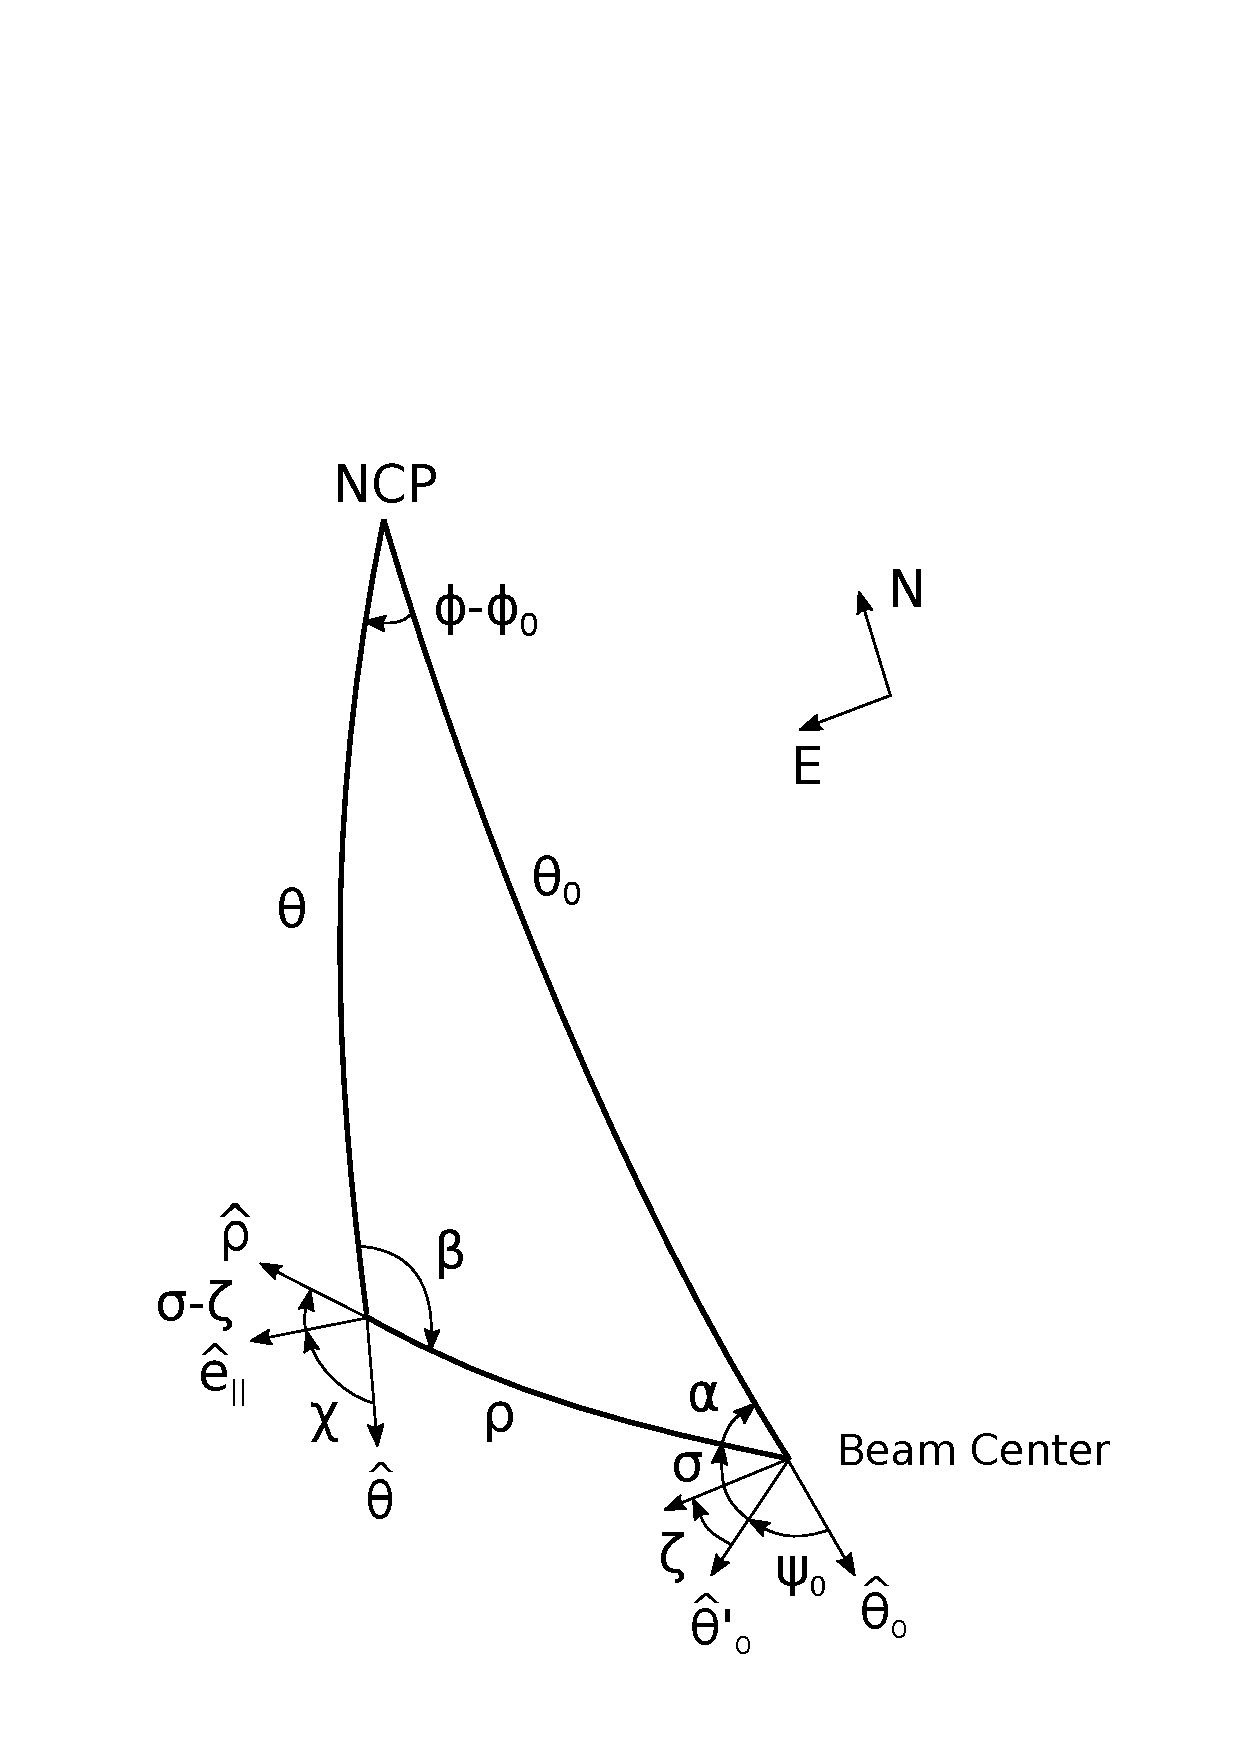
\includegraphics[width=0.8\linewidth]{figures/Figure10_Lu3_3.pdf}
	\caption{Sky and antenna basis coordinates for beam center pointing and off beam center pointing from the viewpoint of an observer looking at the sky. Here $\mathrm{\texttt{NCP}}$ is the 
		     North Celestial Pole and $\chi$ is the angle between $\hat{e}_{\co}$ and $\hat{\theta}$ according to Ludwig's 3rd definition. }
	\label{fig::figure10}
\end{figure}
%
For a beam center pointing $(\theta_0, \phi_0)$, rotation angle $\psi_0$ and off beam center pointing $(\theta, \phi)$ in the sky basis, we can derive the antenna basis coordinates $(\rho,\sigma)$ and the angle $\chi$ between $\hat{e}_{\co}$ and $+Q$ ($\hat{\theta}$) by using spherical trigonometry (see Figure \ref{fig::figure10}). The identities used in this derivation are: the law of cosines, the law of sines and the analogue (or five part) formula.

Defining $\Delta \phi \equiv \phi - \phi_0$, the antenna basis coordinate $\rho$ is given by
%
\begin{align}
\rho  &= \arccos( \cos(\theta) cos(\theta_0) + \sin(\theta) \sin(\theta_0) \cos(\Delta \phi) ).
\end{align}
%
Then, defining $\alpha$ as the angle between $\rho$ and $\theta_0$, the antenna basis coordinate $\sigma$ is given by
%
\begin{align}
\sin(\alpha) &= \frac{\sin(\theta) \sin(\Delta \phi)}{\sin(\rho)} & \\
\cos(\alpha) &= \frac{\cos(\theta) \sin(\theta_0) - \sin(\theta) \cos(\theta_0) \cos(\Delta \phi)}{\sin(\rho)} & \\ 
\alpha       &=  \arctan \left(\frac{\sin(\theta) \sin(\Delta \phi)}{\cos(\theta) \sin(\theta_0) - \sin(\theta) \cos(\theta_0) \cos(\Delta \phi)} \right)  & \\
\sigma &= 180^{\circ} - \psi_0 - \alpha. &
\end{align}
%
Following Ludwig's third definition of cross polarization, substituting $\sigma + 90^{\circ}$ for Ludwig's $\phi$ (see \cite{1140406}), the unit vectors of co and cross polarization for a detector aligned at an angle $\zeta$ with respect to the basis vector $\hat{\theta}'_0$ in the antenna basis are
%
\begin{align}
\hat{e}_{\co} &=  \quad \cos(\sigma - \zeta) \hat{\rho} - \sin(\sigma - \zeta) \hat{\sigma} & \\
\hat{e}_{\cx} &=      - \sin(\sigma - \zeta) \hat{\rho} - \cos(\sigma - \zeta) \hat{\sigma}. & 
\end{align}
%
Thus $\hat{e}_{\co}$ is offset from $\hat{\rho}$ by the angle $\zeta - \sigma$. Then, defining $\beta$ as the angle between $\theta$ and $\rho$, yields
%
\begin{align}
\sin(\beta) &= \frac{\sin(\theta_0) \sin(\Delta \phi)}{\sin(\rho)} & \\
\cos(\beta) &= \frac{\cos(\theta_0) \sin(\theta) - \sin(\theta_0) \cos(\theta) \cos(\Delta \phi)}{\sin(\rho)} & \\ 
\beta       &=  \arctan \left(\frac{\sin(\theta_0) \sin(\Delta \phi)}{\cos(\theta_0) \sin(\theta) - \sin(\theta_0) \cos(\theta) \cos(\Delta \phi)} \right)  & \\
\chi &= \beta + \zeta - \sigma. &
\end{align}
%%
%\section{Calculation of elements of $B$}
%
%A beamsor $B$ evaluated at antenna basis coordinates $(\rho,\sigma)$ is a $4 \times 4$ matrix with elements
%
%\begin{equation}
%\begin{aligned}
%B(\rho,\sigma) = \frac{1}{\tilde{\Omega}}
%\begin{bmatrix}
%B_{TT} & B_{QT} & B_{UT} & B_{VT}\\
%B_{TQ} & B_{QQ} & B_{UQ} & B_{VQ}\\
%B_{TU} & B_{QU} & B_{UU} & B_{VU}\\
%B_{TV} & B_{QV} & B_{UV} & B_{VV}
%\end{bmatrix}
%\end{aligned}
%\label{eq::beamsor_appendix}
%\end{equation}
%
%\noindent
%with $\tilde{\Omega}$ being a normalization factor computed as
%
%\begin{equation}
%\begin{aligned}
%\tilde{\Omega} = \int_{4\pi} B_{TT}(\rho,\sigma) \, \mathrm{d} \Omega
%\end{aligned}
%\end{equation}
%
%The definition of a beamsor used in this work differs from the one listed in \cite{2007MNRAS.376.1767O} in that element $B_{XY}$ corresponds to element $B_{YX}$. We believe this definition yields a clearer interpretation of beamsor elements. Consider, for instance, the product of $B$ with a Stokes vector representing an unpolarized source. This yields
%
%\begin{equation}
%\begin{aligned}
%\begin{bmatrix} 
%B_{TT} \\ 
%B_{TQ} \\ 
%B_{TU} \\ 
%B_{TV} 
%\end{bmatrix}
%=
%\begin{bmatrix}
%B_{TT} & B_{QT} & B_{UT} & B_{VT}\\
%B_{TQ} & B_{QQ} & B_{UQ} & B_{VQ}\\
%B_{TU} & B_{QU} & B_{UU} & B_{VU}\\
%B_{TV} & B_{QV} & B_{UV} & B_{VV}
%\end{bmatrix}
%\cdot
%\begin{bmatrix} 
%1 \\ 
%0 \\ 
%0 \\ 
%0 
%\end{bmatrix}
%\end{aligned}
%\label{eq::unpol_beamsor}
%\end{equation}
%
%\noindent
%where it is more evident that elements $B_{TX}$, with $X=Q,U,V$, correspond to the temperature to polarization leakage beams. 
%
%In most CMB applications, linearly polarized detectors are placed at the focus of the antenna. In general, power that was radiated as pure $+Q$ in the detector basis will reach the sky as both $+Q$ and $-Q$ in the antenna basis. This effect can be modeled by introducing co-polar and cross-polar beams. The co-polar beam, $b_{\co}(\rho,\sigma)$, is the unit-normalized power density distribution that reaches the sky with a polarization state parallel to $\hat{e}_{\co}$. The cross-polar $b_{\cx}(\rho,\sigma)$ does so parallel to $\hat{e}_{\cx}$. 
%
%The work of \cite{2007A&A...470..771J} also provides a way of calculating beamsor elements. Given the coordinate system convention used in this work, it is important to re-specify the way these elements are calculated. We start by considering the antenna to broadcast power originated by a linearly polarized source radiating at the location of the detection device. This will produce a distribution of electric fields in the far field, $\vec{E} = \vec{E}(\rho,\sigma)$, where $\vec{E}(\rho,\sigma)$ will have co-polarized and cross polarized components. Take $x$ to be a source oriented such that most of its radiated power reaches the sky as electric fields aligned with $\hat{\theta}'$ at beam center. Similarly, consider another source, $y$, aligned perpendicularly such that most its transmitted power reaches the sky as electric fields aligned with $\hat{\phi}'$, at beam center. In this situation, elements of a beamsor can be computed via
%
%\begin{equation}
%\begin{split}
%B_{TT}&=\frac{1}{2}\left(\left|\vec{E}_{x}\right|^{2}+\left|\vec{E}_{y}\right|^{2}\right)\\
%B_{QT}&=\frac{1}{2}\left(\left|\vec{E}_{x,\co}\right|^{2}-\left|\vec{E}_{x,\cx}\right|^{2} +  \left|E_{y,\cx}\right|^{2}-\left|E_{y,\co}\right|^{2}\right)\\
%B_{UT}&=\frac{1}{2}\left(\vec{E}_{x,\co} E_{x,\cx}^{*} - E_{y,\co} E_{y,\cx}^{*}\right) + \mathrm{c.c.}\\
%B_{VT}&=\frac{1}{2}\mathrm{i}\left(\vec{E}_{x,\co}\vec{E}_{x,\cx}^{*} + \vec{E}_{y,\co} \vec{E}_{y,\cx}^{*}\right) + \mathrm{c.c.}\\
%B_{TQ}&=\frac{1}{2}\left(\left|\vec{E}_{x}\right|^{2}-\left|\vec{E}_{y}\right|^{2}\right)\\
%B_{QQ}&=\frac{1}{2}\left(\left|\vec{E}_{x,\co}\right|^{2}-\left|\vec{E}_{x,\cx}\right|^{2}+\left|\vec{E}_{y,\co}\right|^{2}-\left|\vec{E}_{y,\cx}\right|^{2}\right)\\
%B_{UQ}&=\frac{1}{2}\left(\vec{E}_{x,\co} \vec{E}_{x,\cx}^{*} + \vec{E}_{y,\co} \vec{E}_{y,\cx}^{*}\right)+\mathrm{c.c.}\\
%B_{VQ}&=\frac{1}{2}\mathrm{i}\left( \vec{E}_{x,\co} E_{x,\cx}^{*} - E_{y,\co} E_{y,\cx}^{*}\right)+\mathrm{c.c.}\\
%B_{TU}&=\frac{1}{2}\left( -\vec{E}_{x,\co} \vec{E}_{x,\cx}^{*} + \vec{E}_{y,\cx} \vec{E}_{y,\co}^{*}\right)+\mathrm{c.c.}\\
%B_{QU}&=\frac{1}{2}\left(-\vec{E}_{x,\co}\vec{E}_{y,\cx}^{*} - \vec{E}_{x,\cx} \vec{E}_{y,\co}^{*}\right)+\mathrm{c.c.}\\
%B_{UU}&=\frac{1}{2}\left(\vec{E}_{x,\co} \vec{E}_{y,\co}^{*} - \vec{E}_{x,\cx} \vec{E}_{y,\cx}^{*}\right)+\mathrm{c.c.}\\
%B_{VU}&=\frac{1}{2}\mathrm{i}\left(\vec{E}_{x,\co} \vec{E}_{y,\co}^{*} + \vec{E}_{x,\cx}\vec{E}_{y,\cx}^{*}\right)+\mathrm{c.c.}\\
%B_{TV}&=\frac{1}{2}\mathrm{i}\left(\vec{E}_{x,\co} \vec{E}_{y,\cx}^{*} - \vec{E}_{x,\cx}\vec{E}_{y,\co}^{*}\right)+\mathrm{c.c.}\\
%B_{QV}&=\frac{1}{2}\mathrm{i}\left(\vec{E}_{\mathrm{x,\co}} \vec{E}_{y,\cx}^{*} + \vec{E}_{x,\cx} \vec{E}_{y,\co}^{*}\right)+\mathrm{c.c.}\\
%B_{UV}&=\frac{1}{2}\mathrm{i}\left(-\vec{E}_{x,\co} \vec{E}_{y,\co}^{*} + \vec{E}_{x,\cx} \vec{E}_{y,\cx}^{*}\right)+\mathrm{c.c.}\\
%B_{VV}&=\frac{1}{2}\left(\vec{E}_{x,\co} \vec{E}_{y,\co}^{*} + \vec{E}_{x,\cx} \vec{E}_{y,\cx}^{*}\right)+\mathrm{c.c.}
%\end{split}
%\end{equation}
%%
%\noindent
%where c.c. stands for complex conjugate.

\end{document}
